\section{Правила игры}

\subsection{Начало игры}

\subsubsection{Игровой набор}

Для игры используются 136 специальных костей, которые чаще называют \textit{тайлами}. Есть 34 вида тайлов, и каждый из них встречается в наборе ровно четыре раза (34 х 4 = 136). На одной стороне тайла находится значимое изображение, другая же, рубашка, у всех тайлов одинакова.

\textbf{Тайлы мастей}:

\noindent\begin{tabular}{ C{3.5cm}ccccccccc } 
	\toprule
	Масть/номинал & 1 & 2 & 3 & 4 & 5 & 6 & 7 & 8 & 9 \\
	\midrule
	Ман \newline & \mahjong{1m} & \mahjong{2m} & \mahjong{3m} & \mahjong{4m} & \mahjong{5m} & \mahjong{6m} & \mahjong{7m} & \mahjong{8m} & \mahjong{9m} \rule[1ex]{0pt}{7ex} \\
	\midrule
	Пин \newline & \mahjong{1p} & \mahjong{2p} & \mahjong{3p} & \mahjong{4p} & \mahjong{5p} & \mahjong{6p} & \mahjong{7p} & \mahjong{8p} & \mahjong{9p} \rule[1ex]{0pt}{7ex} \\
	\midrule
	Соу \newline & \mahjong{1s} & \mahjong{2s} & \mahjong{3s} & \mahjong{4s} & \mahjong{5s} & \mahjong{6s} & \mahjong{7s} & \mahjong{8s} & \mahjong{9s} \rule[1ex]{0pt}{7ex} \\
	\midrule
	Японское чтение & ии & рян & сан & суу & уу & ро & чии & паа & чуу \rule[1ex]{0pt}{2ex} \\
	\bottomrule 
\end{tabular}

\vspace{1cm}

\textbf{Благородные тайлы} (обратите внимание, порядок важен):

\noindent\begin{tabular}{ cC{2cm}C{2cm}C{2cm}C{2cm} } 
	\toprule
	 \rule[0ex]{0pt}{7ex} Ветра & \mahjong{1z} \newline Восток & \mahjong{2z} \newline Юг & \mahjong{3z} \newline Запад & {\mahjong{4z} \newline Север} \\
	\midrule
	Японское чтение & тон & нан & ся & пей \\
	\bottomrule
\end{tabular}

\vspace{1cm}

\noindent\begin{tabular}{ cC{2cm}C{2cm}C{2cm} } 
	\toprule
	 \rule[0ex]{0pt}{7ex} Драконы & \mahjong{5z} \newline Белый & \mahjong{6z} \newline Зеленый & \mahjong{7z} \newline Красный \\
	\midrule
	Японское чтение & хаку & хацу & чун \\
	\bottomrule
\end{tabular}

\pagebreak

Для подсчета очков в игре используются палочки следующих номиналов:

\noindent\begin{tabular}{ ccc } 
	\toprule
	
\includegraphics{tenbo10000} & 10000 очков & x1 \\
	
\includegraphics{tenbo5000} & 5000 очков & x2 \\
	
\includegraphics{tenbo1000} & 1000 очков & x9 \\
	
\includegraphics{tenbo100} & 100 очков & x10 \\
	\bottomrule
\end{tabular}

Иногда можно встретить в наборах палочки номиналом 500 очков, обычно они выглядят так же, как палочки на 100 очков, но окрашенные в зеленый цвет.

Общее количество очков в начале игры у каждого игрока равно 30000. Количество палочек в наборе может также отличаться, например может быть три палочки по 5000 и четыре по 1000, главное чтобы общее количество соответствовало указанному.

Также в игре используются:
\begin{itemize}
	\item Индикатор первого дилера --- небольшая пластинка с изображением восточного ветра (\textnihon{東}) с одной стороны и южного ветра (\textnihon{南}) с другой;
	\item Два шестигранных кубика с цифрами от 1 до 6.
\end{itemize}

\subsubsection{Подготовка к игре}

В риичи-маджонг играют вчетвером. Для игры используют небольшой квадратный стол (\sim75х75 см), с каждой стороны которого садится по игроку. Каждому месту за столом присваивается условная сторона света, и расположены они в порядке тайлов ветров против часовой стрелки: восток (\textnihon{東}), юг (\textnihon{南}), запад (\textnihon{西}), север (\textnihon{北}), т. е. порядок "неправильный" и отличается от настоящего расположения сторон на карте мира\footnote{Порядок ветров соответствует расположению сторон света на карте звездного неба.}. Выбор мест производится по договоренности или по жребию: на стол кладутся четыре разных тайла ветров рубашкой вверх, игроки берут их по очереди, и каждый занимает соответствующее место. Ветер, соответствующий месту игрока, называется \textit{ветром места}. 

Игрок, вытянувший восток, становится первым \textit{дилером} в игре и рядом с ним в начале игры кладется индикатор первого дилера. Обычно дилер выбирает место за столом, остальные рассаживаются относительно него согласно вытянутым ветрам.

Игра делится на раунды, также названные по сторонам света --- восточный (первый) и южный (второй), и раздачи. Существует два варианта партий:
\begin{itemize}
	\item короткая игра, где играется только восточный раунд, называется \textit{тонпусен};
	\item длинная игра, и с восточным, и с южным раундом --- \textit{ханчан}.
\end{itemize}
Ветер, соответствующий текущему раунду, называется \textit{ветром раунда}. Раунд по умолчанию состоит из четырех раздач (хотя в отдельных случаях, оговоренных правилами, могут назначаться дополнительные раздачи), и каждую новую раздачу происходит сдвиг сторон света за столом на одно место против часовой стрелки: игрок, в первой раздаче бывший на юге, во второй оказывается дилером, в третьей --- севером и т. д, сами игроки при этом не пересаживаются. Таким образом, смена раунда происходит, когда дилерство возвращается к игроку, бывшему дилером в первой раздаче. Индикатор первого дилера все время остается лежать рядом с дилером первой раздачи; во время восточного раунда он повернут вверх стороной, где нарисован иероглиф востока, а с началом южного переворачивается. Для указания на дилера текущей раздачи с его стороны стола после подготовки к раздаче кладутся кубики.

Перед началом каждой раздачи игроки кладут все тайлы на стол рубашкой вверх и тщательно их перемешивают. После этого каждый игрок строит перед собой "стену" высотой в 2, шириной в 1 и длиной в 17 тайлов рубашкой вверх, размещая ее так, чтобы в итоге четыре участка стены от разных игроков образовали замкнутый квадрат. Затем дилер бросает кубики и отсчитывает против часовой стрелки столько сторон квадрата, сколько выпало на кубиках суммарно, начиная со своей стороны (на рис.1 показан пример для выпавшей суммы 8).

\begin{figure}[H]
	\centering
	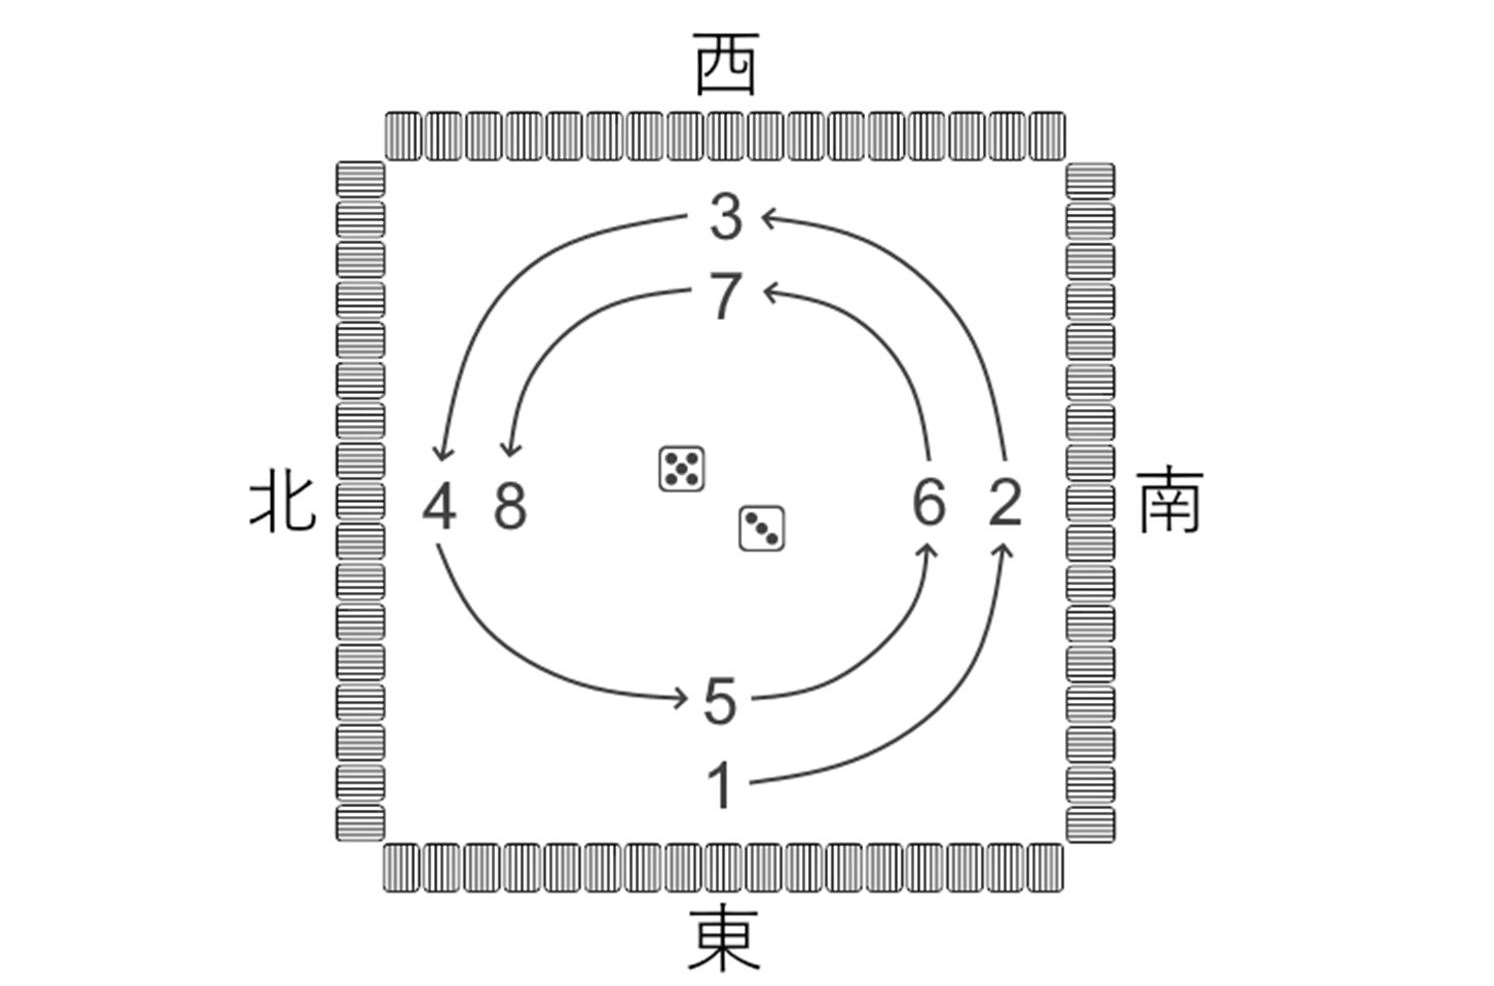
\includegraphics[width=16cm]{table-deal-start.png}
	\caption{Определение разлома стены}
\end{figure}

Затем игрок, на чью сторону указал дилер (в примере выше --- север), отсчитывает от правого конца своей стороны стены столько тайлов, какое число выпало на кубиках до этого (в примере --- 8) и немного отодвигает их от соседних тайлов вправо, создавая разлом стены. После этого он отсчитывает от разлома в обратную сторону 7 тайлов и немного отодвигает получившуюся группу из 14 тайлов\footnote{Для опытных игроков подобное обособление мертвой стены считается излишним, поэтому рекомендуется не отодвигать мертвую стену от живой в самом начале игры, но можно это сделать ближе к концу раздачи. Подробнее см. в разделе про игровой этикет} (см. рис.2). Эта группа называется мертвой стеной и не разбирается\footnote{За исключением одного особого случая при объявлении кана, см. далее} в процессе игры. Оставшаяся часть стены называется живой стеной и используется во время раздачи для получения игроками тайлов (наподобие колоды карт). Разбирается она стопками верхний-нижний по часовой стрелке, начиная с верхнего тайла первой стопки после разлома и заканчивая нижним последней перед мертвой стеной. Стена считается непрерывной, и переход через углы не имеет никакого значения как при формировании мертвой стены, так и при последующем разборе.

Допускается формирование первого разлома стены дилером при первом взятии, однако, поскольку такой способ может приводить к ошибкам в разборе стены, на турнирах мы его рекомендовать не можем.

Третий верхний тайл от конца мертвой стены переворачивается рубашкой вниз (на рисунке это 6 ман) и служит в данной раздаче индикатором доры --- тайла, дающего дополнительные очки при его наличии в руке. Подробно о дорах и принципе работы индикаторов рассказано в разделах далее.

\begin{figure}[H]
	\centering
	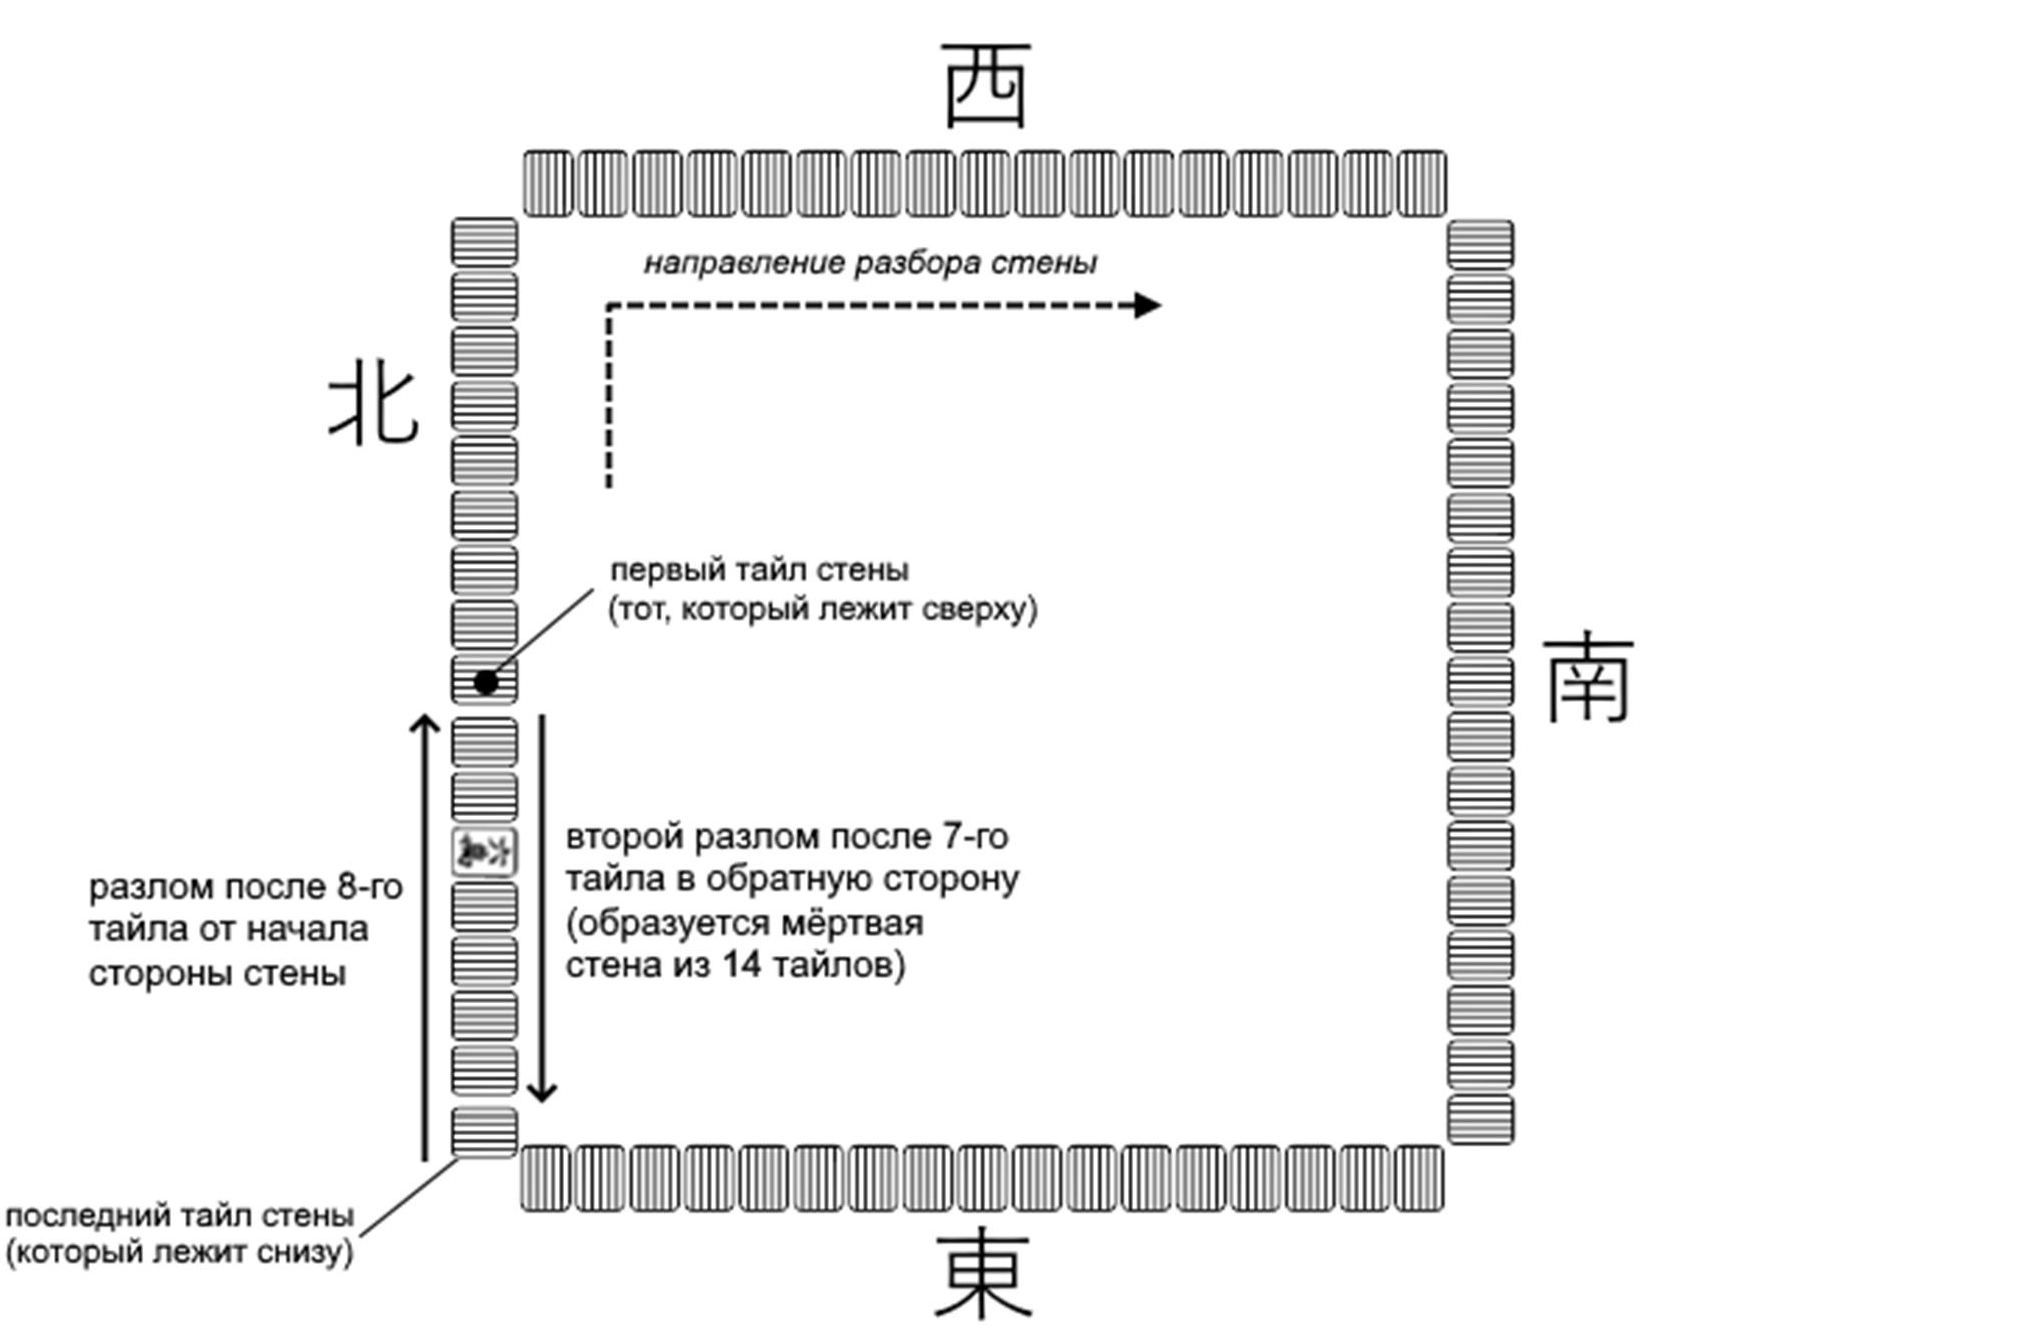
\includegraphics[width=16cm]{table-deal-start-2.png}
	\caption{Мертвая и живая стены}
\end{figure}

После открытия индикатора доры игроки начинают набор своих стартовых рук со стены\footnote{Допускается открыть индикатор доры после того как руки набраны, но нужно это сделать до первого сброса дилера}. Начиная с дилера по очереди против часовой стрелки игроки начинают брать от начала живой стены по четыре тайла (две стопки по 2), пока у каждого не окажется 12 тайлов.
После этого дилер берет один крайний тайл со стены и тайл через один от него, далее игрок на юге берет нижний тайл, игрок за западе - верхний тайл перед тем, который уже взял дилер, и игрок на севере забирает один оставшийся тайл.

Таким образом, в начале раздачи дилер имеет 14 тайлов, а остальные --- по 13. Тайлы своих рук игроки расставляют перед собой в ряд вертикально изображением к себе, так, чтобы остальные видели только их рубашки. Сортировка тайлов в руке оставляется на усмотрение игрока, однако в случае показательных игр (например, при игре на камеру) сортировка руки является рекомендуемой.

\begin{figure}[H]
	\centering
	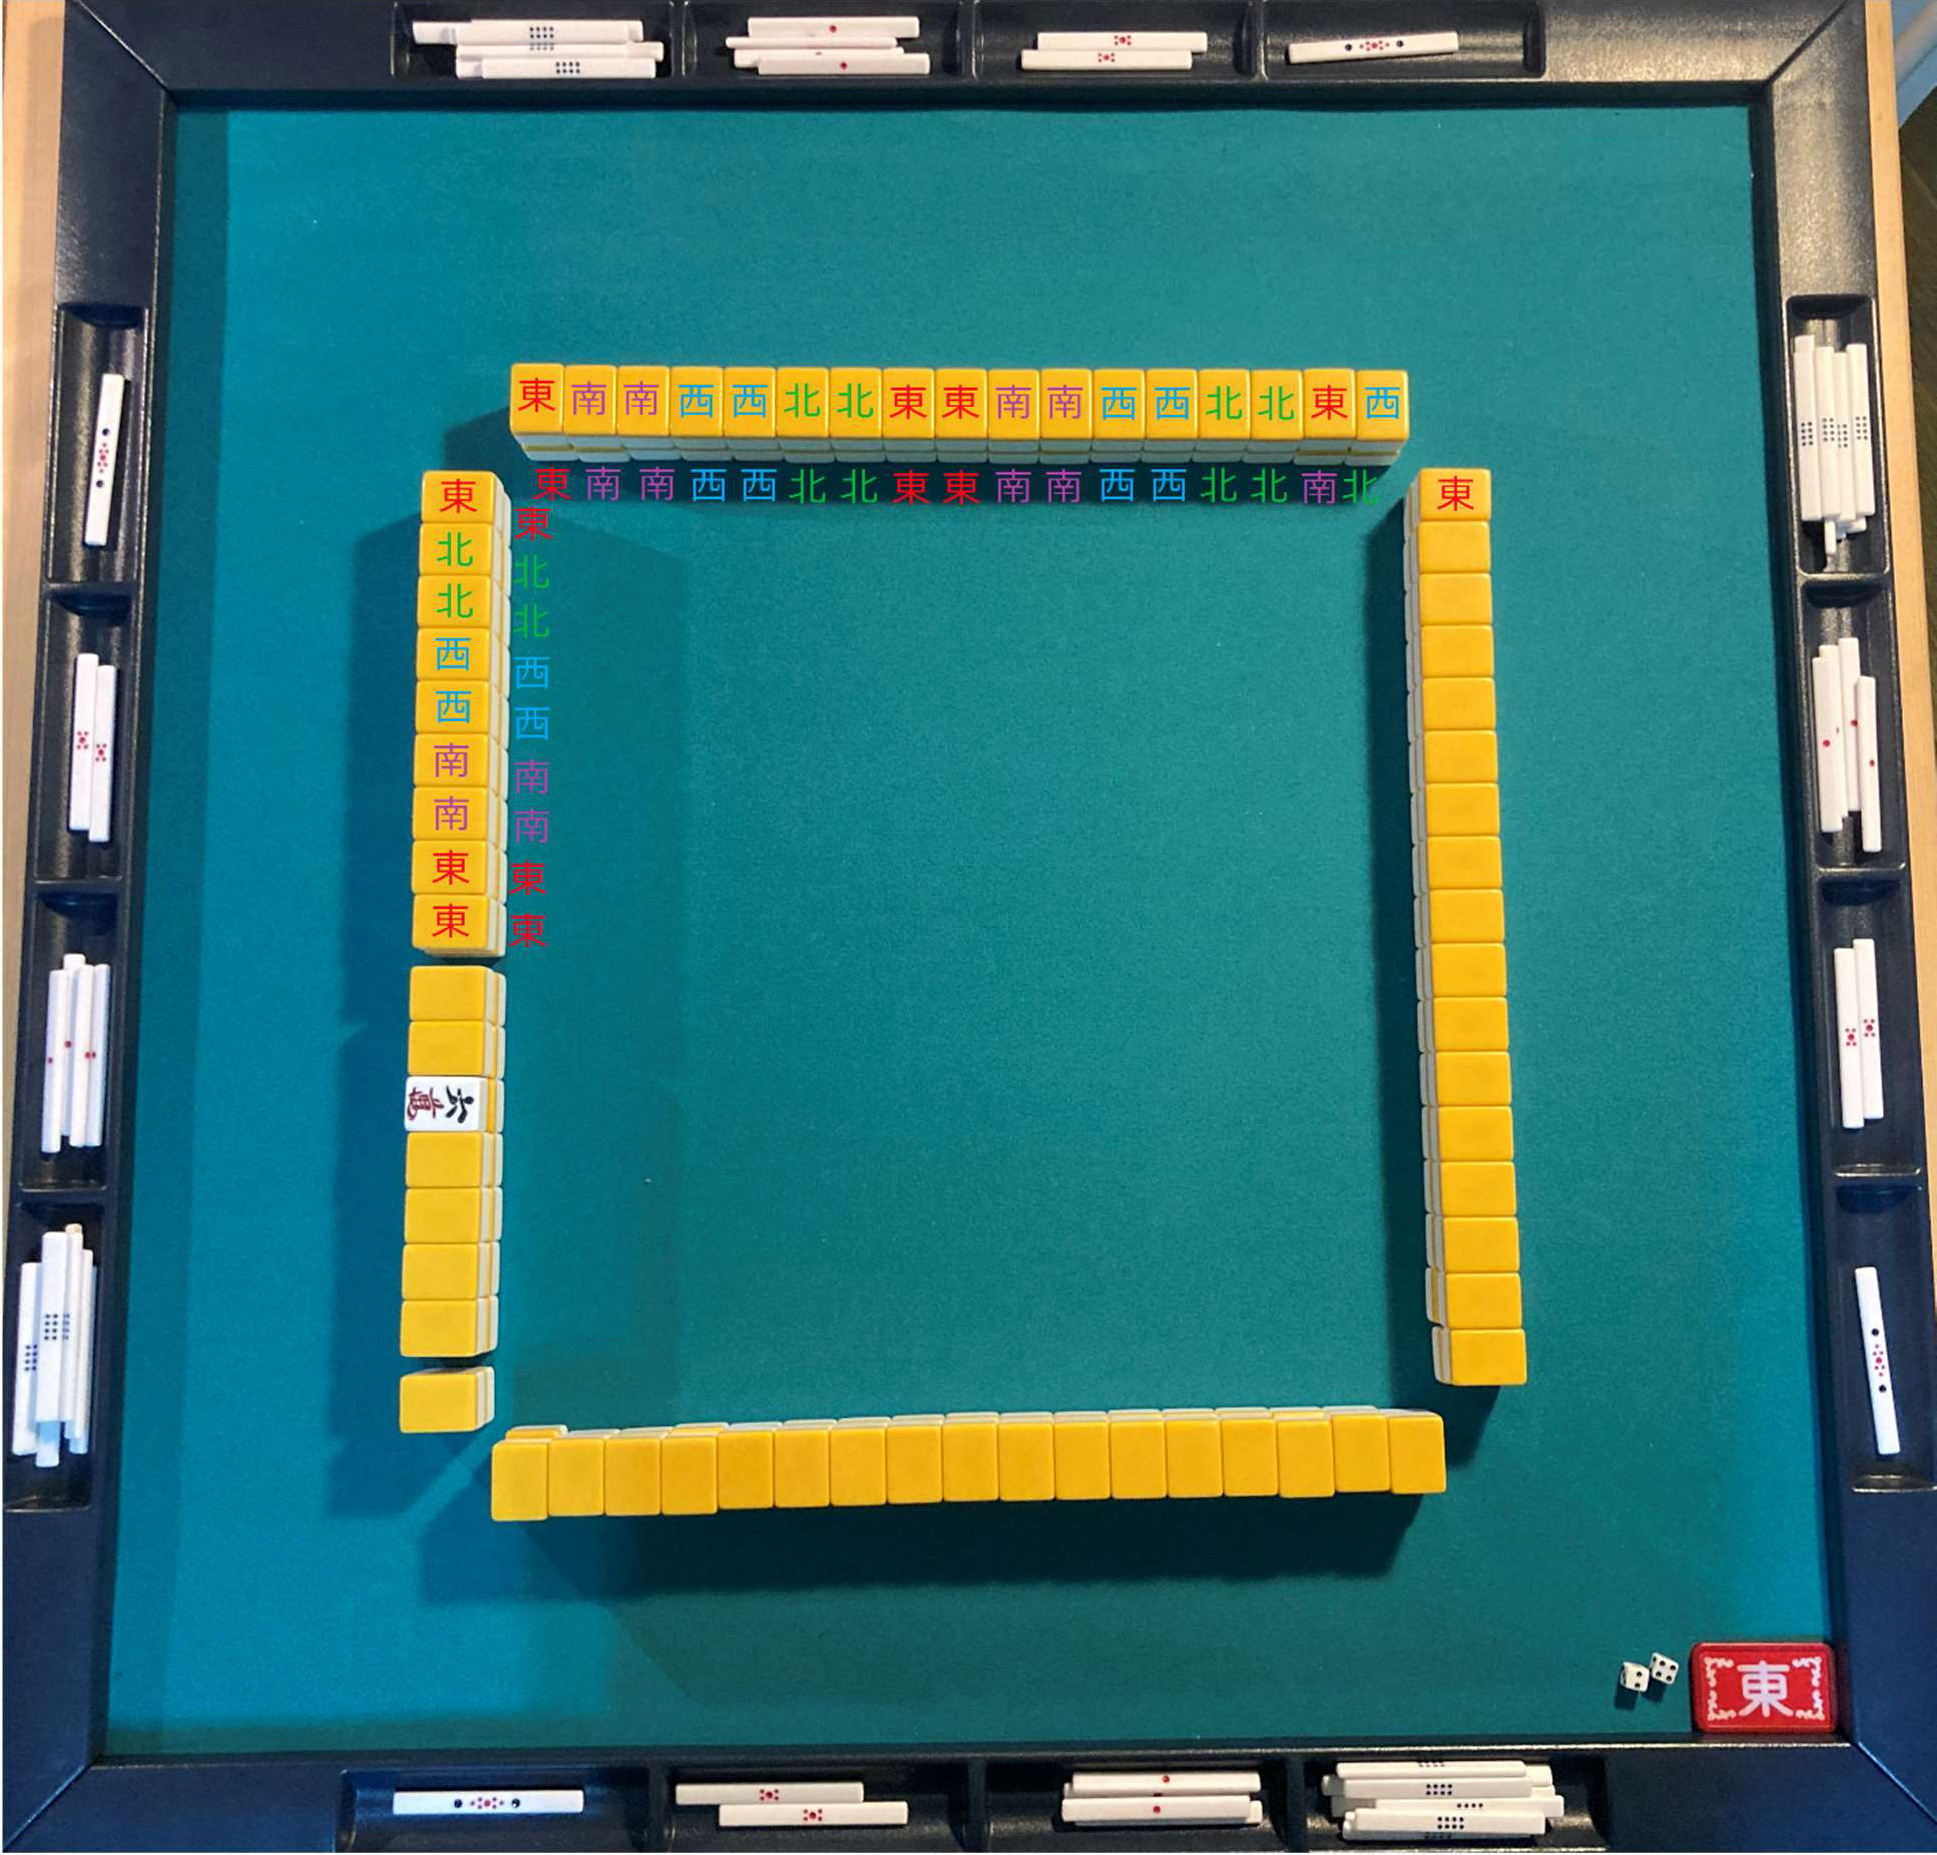
\includegraphics[width=16cm]{table-deal-start-3.png}
	\caption{Порядок разбора стены, фото}
\end{figure}

Обратите внимание на подписи тайлов --- они показывают, какой игрок должен их взять (верхние тайлы стены подписаны прямо на рубашке, нижние --- рядом). Предположим, что сейчас идет первая раздача восточного раунда: на индикаторе первого дилера указан восток, а кубики, как индикатор текущего дилера, лежат рядом с ним, т. е. первый дилер является дилером в этой раздаче.

\subsection{Ход раздачи}

В ходе раздачи, которая начинается сразу же после набора и сортировки всеми стартовых рук, игроки изменяют состав своих рук, набирая в них по одному новые тайлы с живой стены и выбрасывая ненужные. Цель каждого игрока в раздаче --- собрать в руке четыре сета и одну пару (два одинаковых тайла). При объявлении кем-либо победы с готовой рукой раздача заканчивается. Цель всей игры --- набрать как можно больше очков.

Сет --- это определенная комбинация из трех или четырех тайлов. Они бывают трех видов:
\begin{itemize}
	\item Три одинаковых тайла --- \textit{пон};
	\item Четыре одинаковых тайла --- \textit{кан} (должен быть \textit{объявлен}, про объявления см. далее);
	\item Последовательность из трех тайлов одной масти подряд (по типу 1-2-3, 3-4-5 и т. п.) --- \textit{чи}. Последовательности можно собирать только из тайлов мастей, и в них не должно быть перехода через девятку: 8-9-1 и 9-1-2 не засчитываются как чи.
\end{itemize}

Один тайл не может одновременно входить в два сета. В примере ниже в руке уже есть готовый пон из 4 ман, чи 7-8-9 ман и пара красных драконов, но последовательность 3-4-5-6-7 пин не засчитывается за два чи: для завершения этой формы в два сета требуется получить еще один тайл (2, 5 либо 8 пин).

\mahjong{444789m 34567p 77z}

В руке из примера выше 13 тайлов, как и в любой руке не-дилера в начале раздачи, но выигрышная рука должна содержать как минимум 14 тайлов (3+3+3+3+2, если же в руке есть каны, число тайлов может доходить до 18). Четырнадцатый тайл игроки получают в свои ходы во время раздачи: раздача начинается с хода дилера, который сбрасывает из руки один из своих 14 тайлов, кладя его рубашкой вниз в центр стола; затем ход переходит к следующему игроку против часовой стрелки, который берет первый тайл из оставшейся части живой стены и также сбрасывает один тайл из своей руки (можно сбрасывать и тайл, только что взятый со стены --- такой сброс называется \textit{цумогири}). Затем ход переходит к следующему игроку. Так раздача продолжается до тех пор, пока кто-либо не соберет руку и объявит победу, или же пока в живой стене не закончатся тайлы. 

Ходы в риичи-маджонге обязательны, пропускать взятие со стены либо сброс нельзя. Каны, а вместе с ними и руки, содержащие более 14 тайлов, возможно образовать специальными объявлениями, о которых рассказывается в следующем разделе. Ходы четырех игроков, начиная от дилера, образуют круг раздачи. После окончания круга ход вновь переходит к дилеру, и начинается следующий круг. Группы сброшенных тайлов в центре стола называются сбросами или \textit{дискардами}. Каждый игрок имеет свой отдельный дискард. Тайлы следует выкладывать в сброс слева направо тремя рядами по 6 штук (начиная с ближнего к центру стола и далее по направлению к себе); четвертый же ряд чаще не начинают, а вместо этого продолжают третий.

Нельзя забрать только что сброшенный тайл обратно в руку и сбросить другой - подобное нарушение карается мертвой рукой.

\begin{figure}[H]
	\centering
	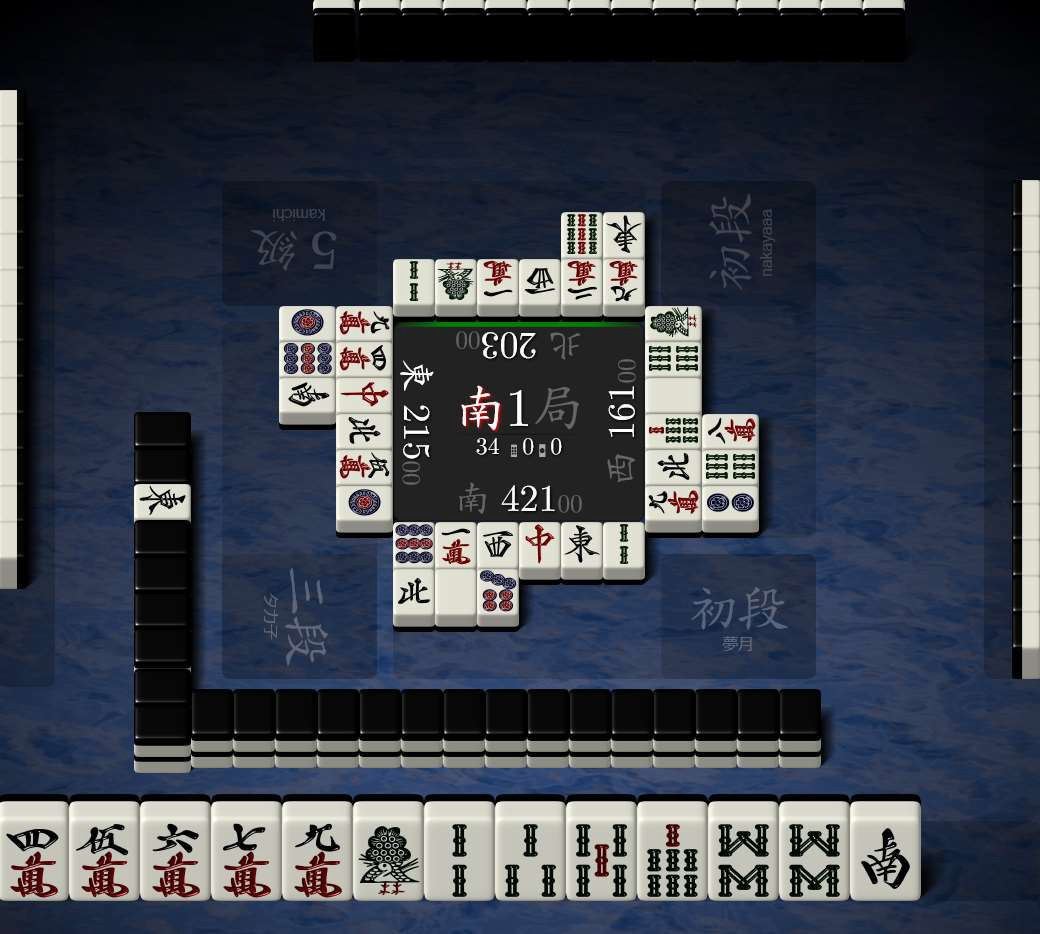
\includegraphics[width=16cm]{tenhou-deal.jpg}
	\caption{Пример раздачи на сервере tenhou.net}
\end{figure}

Рассмотрим вид стола в процессе раздачи на онлайн-сервере tenhou.net (рис.4). В центре --- указатель раунда, номера раздачи в раунде (южный, первая) и указатели мест игроков со счетчиками очков (мы юг с 42100 очков; на онлайн-серверах вместо палочек используются цифровые счетчики). Вокруг центра --- дискарды игроков, ниже --- живая стена, слева --- мертвая стена с индикатором доры восточным ветром. По краям стола расположены руки игроков. Сейчас 9-й круг, ход севера: он получил тайл со стены, но еще не совершил сброс. Пришедший со стены тайл обычно сначала ставят отдельно от руки и встраивают в руку только после сброса, если сброшен другой тайл. См. подробнее про порядок взятий в разделе про игровой этикет.

\subsection{Объявления в игре}

Помимо взятий со стены и сбросов во время раздачи игроки могут делать различные \textit{объявления}. Основных видов объявлений два: это объявления на тайлы (объявления сетов) и объявления победы. Помимо этого, существует отдельное объявление абортивной ничьей и особое объявление риичи, но о них рассказывается в соответствующих разделах.

Объявления на тайлы позволяют ускорить сбор руки, используя для завершения сетов тайлы, сбрасываемые другими игроками. Объявить сет с чужим сброшенным тайлом можно только в момент его сброса другим игроком и до взятия со стены тайла следующим игроком --- после этого тайл в дискарде считается вышедшим из игры, и больше его использовать для объявлений нельзя. Нельзя также делать объявления и на последний сбрасываемый тайл за раздачу, когда в живой стене не остается тайлов. 

Рука, в которой есть объявленные сеты с чужими тайлами, называется \textbf{открытой}, а рука без них --- \textbf{закрытой}. Сет, образованный любым объявлением, считается фиксированным, и изменять его нельзя. Сбросы разрешается делать только из оставшейся закрытой части руки.

\subsubsection{Объявление "пон" (\textnihon{ポン})}

\textbf{Пон} --- это три одинаковых тайла. Объявление пона позволяет дополнить имеющиеся в руке два одинаковых тайла третьим таким же тайлом, когда его сбрасывает другой игрок. Пон можно объявить на тайл, сброшенный любым из трех противников. Объявление пона приоритетнее, чем объявление чи (см. далее) на тот же сброшенный тайл. Последовательность действий при объявлении такова:

\begin{itemize}
	\item После сброса нужного тайла противником в дискард нужно сказать "пон";
	\item Затем следует выложить свою пару тайлов плашмя рубашкой вниз справа от руки;
	\item После этого нужно взять тайл из дискарда противника и положить его боком слева, между или справа от тайлов пары в зависимости от того, с игрока слева, напротив или справа был взят пон. Выглядит это так (поны с игроков слева, напротив и справа соответственно):
\end{itemize}

\mahjong{4'44m-55'5m-666'm}

Например, рука

\mahjong{22345m 237p 4888s 2z}

после взятия 2 ман с игрока напротив будет выглядеть так:

\mahjong{345m 237p 4888s 2z} \hfill \mahjong{22'2m}

При этом тайлы в закрытой части руки остаются стоять вертикально, тогда как тайлы дополненного сета лежат плашмя и видны всем.

Наконец, после объявления сбрасывается тайл из закрытой части руки, и ход переходит к следующему игроку от взявшего пон против часовой стрелки, т. е. объявление нарушает порядок ходов, прерывая круг.

\subsubsection{Объявление "чи" (\textnihon{チー})}

Чи --- это сет, образованный любыми тремя тайлами одной и той же масти в непрерывающейся последовательности (например, 4-5-6). Чи нельзя собрать из благородных тайлов, кроме того замыкающаяся через краевые тайлы последовательность также не считается как чи (например, 9-1-2 --- это не чи).

Если в руке есть два любых тайла, которые могут входить в одну последовательность, при сбросе противником третьего тайла этой последовательности объявлением "чи" можно дополнить эти два тайла до чи. Чи можно объявлять только на тайлы, сброшенные игроком слева. Последовательность действий при объявлении "чи" такая же, как и при объявлении "пон":

\begin{itemize}
	\item После сброса игроком слева тайла в дискард нужно сказать "чи";
	\item Затем следует выложить два тайла последовательности из руки плашмя рубашкой вниз справа;
	\item После этого нужно взять тайл из дискарда противника и дополнить им последовательность, положив взятый тайл боком слева от двух открытых тайлов;
	\item Наконец, следует осуществить сброс тайла из руки.
\end{itemize}

Отметим, что в клубных играх может допускаться сброс тайла из руки до того, как будет взят тайл из дискарда. Это позволяет несколько ускорить игровой процесс, однако на турнирных играх такое не приветствуется и может быть наказано вежливым указанием так не делать, со штрафом при повторении.

Взятый при "чи" тайл всегда кладется слева от двух других, даже если при этом нарушается порядок последовательности. Если с рукой из примера выше, где уже взят пон на 2 ман, взять на следующем круге чи при сбросе игроком слева 4 пин, она будет выглядеть так:

\mahjong{345m 7m 4888s} \hfill \mahjong{4'23p-22'2m}

(предположим, что южный ветер был сброшен после объявления пона на 2 ман). Каждый следующий объявленный сет кладется слева либо сверху от предыдущего.

\subsubsection{Объявление "кан" (\textnihon{カン})}

"Кан" --- объявление, позволяющее создавать в руке каны, одноименные сеты из четырех одинаковых тайлов. Если в закрытой части руки есть четыре одинаковых тайла, но кан не был объявлен, они не интерпретируются как кан (поскольку иначе в руке не хватит тайлов для четырех сетов и пары), но могут интерпретироваться любым другим способом. Например, в руке ниже кан не объявлен, и поэтому четыре тайла 5 ман не считаются за кан, но могут считаться за пон и часть чи 5-6-7, либо за пару, часть чи и свободный тайл и т.д.

\mahjong{555567m 1p 99s 3356z}

Кан можно объявлять тремя различными способами.

\textbf{Закрытый кан (\textit{анкан})}

Если игрок имеет в закрытой части руки четыре одинаковых тайла, он в любой свой ход после взятия тайла со стены, но до сброса, может сказать "кан" и выложить эти четыре тайла плашмя справа, положив два крайних тайла рубашкой вверх, а два средних --- рубашкой вниз (крайние тайлы следует предварительно показать противникам). С закрытым каном 5 ман из руки выше это будет выглядеть так:

\mahjong{67m 1p 99s 3356z} \hfill \mahjong{X55mX}

Закрытый кан нельзя объявлять сразу после своего объявления чи или пона (но можно после другого кана). Рука с закрытым каном продолжает считаться закрытой --- это единственный объявляемый сет-исключение.

\textbf{Открытый кан (\textit{дайминкан})}

Если у игрока в закрытой части руки есть три одинаковых тайла, и любой противник сбрасывает четвертый, он может объявить на него "кан", действуя точно так же, как и при объявлении "пон". Тайлы кана кладутся плашмя справа таким же образом, как и после "пона". Если кан был взят с игрока напротив, можно повернуть боком любой из двух средних тайлов. Пример: если игрок из примеров выше, до этого взявший пон и чи, берет на следующем после чи круге кан 8 соу с игрока справа, его рука будет выглядеть как на схеме ниже.

\mahjong{345m 7m} \hfill \mahjong{8888's-4'23p-22'2m}

(предположим, что 4 соу была сброшена после объявления чи). Объявление кана приоритетнее объявления чи на тот же сброшенный тайл.

\textbf{Дополненный кан (\textit{шоминкан})}

Если у игрока есть открытый пон и четвертый такой же тайл в закрытой части руки, в любой свой ход после взятия со стены и до своего сброса он может дополнить пон до кана объявлением "кан". Четвертый тайл кладется боком сверху от тайла, лежавшего боком в поне. Такой кан, как и закрытый, нельзя объявлять сразу после своего объявления "чи" или "пон" (но можно после другого любого кана). Дополненный кан считается открытым, поскольку условием для его появления служит наличие открытого пона в руке, соответственно, рука всегда уже открыта на момент появления такого кана.

% TODO: ошибка при компиляции, но на самом деле не ошибка; раскомментить
\mahjong{22"2m}

После объявления любого кана в закрытой части руки начинает не хватать тайлов для ее завершения, и поэтому игрок сразу же должен взять в руку тайл замены (\textit{риншанпай})\footnote{крайний тайл с того конца мертвой стены, около которого находится разлом}, и только потом совершить сброс. Это единственная ситуация в игре, когда берутся тайлы с мертвой стены. Кроме того, при объявлении каждого кана открывается один индикатор кандоры: переворачивается соседний с индикатором доры верхний тайл с "длинной" стороны мертвой стены. Новый индикатор открывается \textit{сразу} после объявления и до взятия игроком дополняющего тайла с мертвой стены\footnote{В некоторых правилах, особенно в онлайн-маджонге, новый индикатор открывается сразу только в случае объявления закрытого кана, если же кан открытый, новый индикатор открывается только после сброса}. Дополняющий тайл может быть затребован для победы как обычный дискард, в таком случае новый индикатор не открывается, так как кан фактически не был объявлен.

Ход после объявления кана, открытия кандоры и сброса переходит следующему игроку против часовой стрелки от объявившего, как и при других объявлениях сетов. 

В мертвой стене всегда должно сохраняться 14 тайлов. Поэтому при взятии тайла замены последний тайл живой стены условно\footnote{"Условно" значит, что тайлы не перекладывают в мертвую стену, просто раздача при отсутствии победителя заканчивается раньше на столько тайлов живой стены, сколько за столом открыто канов. Из-за того, что в раздачах с канами второй разлом не показывает конец живой стены, за некоторыми столами его по договоренности могут не делать, считая ненужным, см. раздел про этикет за столом.} докладывается в мертвую стену, и живая стена укорачивается на один тайл с конца.

Всего за раздачу может быть объявлено не более чем 4 кана: именно столько тайлов замены возможно взять с короткого конца мертвой стены, и столько индикаторов кандор можно открыть с длинного. В случае открытия четырех канов разными игроками, после объявления четвертого кана и сброса тайла, на котором в итоге никто из игроков не объявляет победу, объявляется абортивная ничья (см. раздел про ничьи далее). Если все четыре кана открыты одним и тем же игроком, игра продолжается, но игроки не вправе объявить пятый кан.

\begin{figure}[H]
	\centering
	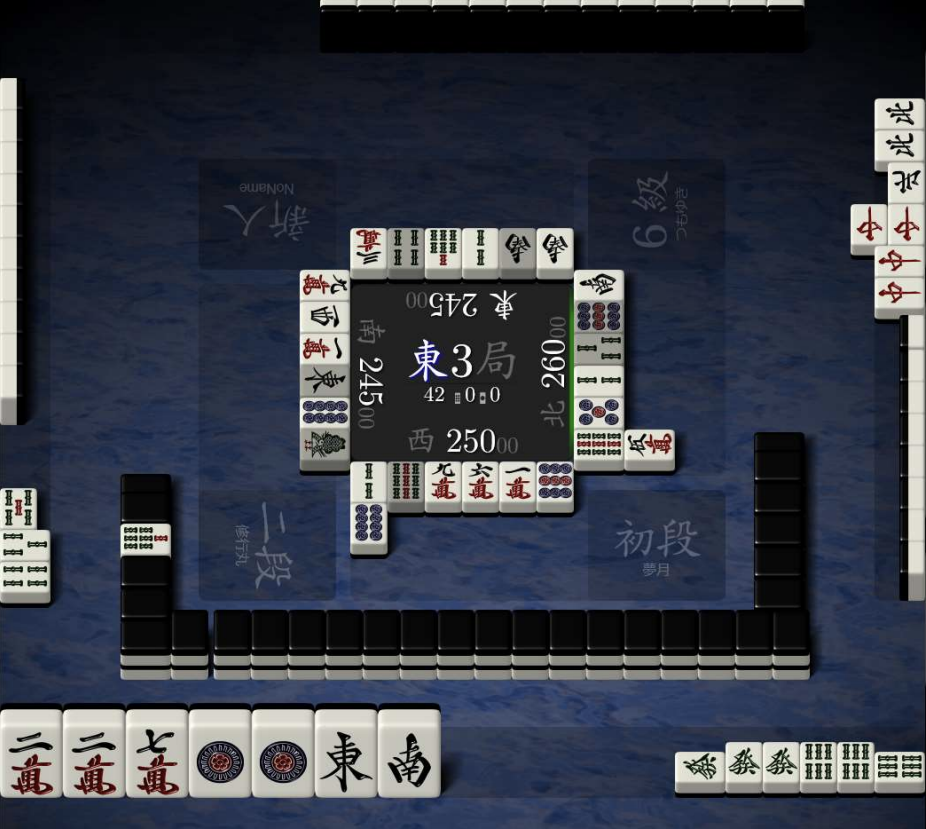
\includegraphics[width=16cm]{tenhou-sets}
	\caption{Пример сетов}
\end{figure}

Рассмотрим стол на tenhou.net c различными открытыми сетами. Мы запад, объявили пон 6 соу с игрока справа, а затем пон зеленых драконов с игрока слева. Сам игрок слева объявил чи на 5 соу в последовательность 3-4-5. Игрок напротив играет с закрытой рукой. Игрок справа объявил пон северных ветров с нас, затем пон красных драконов с дилера, а текущим ходом дополнил его до кана. Сейчас он уже взял тайл замены --- он у него в закрытой части руки самый верхний (если присмотреться, видно, что в мертвой стене нет одного верхнего тайла с короткого конца), но еще не сделал сброс.

Схема мертвой стены: все тайлы в ней, кроме докладываемых из живой стены при объявлении канов, могут использоваться в раздаче как тайлы замены либо как индикаторы дор (урадоры и кан-урадоры могут вводиться в игру после объявления риичи, см. далее про доры). После объявления первого кана за раздачу берется первый тайл замены, открывается первый индикатор кандоры и 1-й тайл с конца живой стены становится частью мертвой стены, после второго кана эти действия производятся со вторыми тайлами и т. д. 

\subsubsection{Куикаэ}

В данных правилах регламентируется так называемое правило \textit{куикаэ} --- оно определяет, можно ли осуществлять сброс такого же тайла после взятия сета, можно ли осуществлять сброс тайла, ранее дополнявшего до последовательности объявляемые два тайла, или оба действия недопустимы --- последний вариант регламентируется как обязательный. В случае нарушения данного правила, игроку назначается мертвая рука, но никаких изменений в дискарде делать не следует (т.е. нельзя забрать тайл обратно и скинуть другой тайл). Пример:

\mahjong{2255m 5678s 333z} \hfill \mahjong{5'34m}

Сброс как 2 ман, так и 5 ман в данном случае недопустим из-за правила куикаэ. Аналогичным образом, после взятия пона не допускается сброс такого же тайла, какой был взят в пон.

\subsubsection{Объявления победы}

Когда игроку не хватает в руке до победы (также называемой \textit{агари}), одного тайла (такое состояние руки называется \textit{темпай}), он может выиграть раздачу, получив выигрышный тайл двумя способами:

\begin{itemize}
	\item Со стены в свой ход. Такая победа называется цумо (\textnihon{ツモ}), и объявляется словом "цумо" после взятия выигрышного тайла.
	\item При сбросе другим игроком на его ходу. Такая победа называется рон (\textnihon{ロン}) и объявляется словом "рон".
\end{itemize}

В случае, если \textit{все без исключения} возможные выигрышные тайлы уже находятся в руке игрока (в закрытой части и в объявленных сетах), темпай не засчитывается.

Пример темпая:

\mahjong{23455m 34p 456s} \hfill \mahjong{7'68m}

Выигрышные тайлы, завершающие руку в четыре сета и пару --- 2 и 5 пин. Игрок может объявить цумо, если один из них зайдет со стены, или рон, если какой-то из них сбросит любой противник. После объявления цумо выигрышный тайл кладется рядом с рукой, а рука показывается игрокам. Класть выигрышный тайл в руку при цумо не следует, потому что в некоторых случаях для определения стоимости руки имеет значение, с какого именно тайла игрок выиграл раздачу. При роне брать выигрышный тайл из дискарда сбросившего игрока не следует, рука также показывается противникам.

Обратите внимание, что выигрышный тайл нельзя класть в зону дискарда. Если тайл выложен в дискард --- объявлять победу по цумо на нем недопустимо. Предполагается, что игрок понимает свое ожидание и знает, какие именно тайлы дают ему победу. В случае сомнения допускается недолго подумать перед сбросом.

Объявление победы завершает раздачу. После показа руки производится подсчет очков и выплата за руку, и затем, если раздача не была последней, начинается следующая. Объявления победы, как и объявления сетов, не обязательны:
\begin{itemize}
	\item рон можно пропустить, или сделать на этот тайл другое объявление --- пон, кан или чи;
	\item цумо тоже можно не объявлять, сбросив любой тайл из руки после получения выигрышного и продолжив раздачу.
\end{itemize}
Однако такие пропуски накладывают на дальнейшие возможности победы некоторые ограничения из-за правила фуритен, рассмотренного далее.

Несколько игроков в темпае могут объявить рон на один и тот же сброшенный тайл одновременно. В этом случае выплаты производятся каждому из победивших игроков. 

Также рон можно объявить во время объявления противником дополненного кана, когда противник дополняет пон выигрышных для игрока тайлов четвертым тайлом, а в одном очень редком специфическом случае --- и при объявлении противником закрытого кана (см. раздел про яку). При "роне с кана", который также называют перехватом тайла или ограблением кана, набросившим считается игрок, объявивший кан. При ограблении кана кан не считается объявленным, следовательно новый индикатор доры не открывается (про доры см. далее).

Не рекомендуется объявлять пон исходя из того, что кто-то решил взять чи. Подробнее см. также в разделе про игровой этикет.

Когда разные игроки одновременно делают различные объявления на один тайл, забирает его тот игрок, чье объявление приоритетнее:

\begin{itemize}
	\item Пон или кан приоритетнее чи;
	\item Рон приоритетнее, чем пон или кан.
\end{itemize}

Последний момент, когда можно объявить рон --- сброс следующего по ходу игры игрока. После того, как этот сброс осуществлен и следующий игрок взял тайл, объявление победы не допускается. Однако, рекомендуется внимательно следить за ходом игры и объявлять победу сразу же. В случае, если игроки делают сбросы и взятия слишком быстро, следует попросить игроков делать небольшие паузы.

\subsubsection{Риичи}

Риичи (\textnihon{リーチ} от англ. “reach”) --- одно из самых частых условий победы, встречающихся в риичи-маджонге, давшее ему первую часть названия. Это объявление, позволяющее выиграть на любой закрытой руке, находящейся в темпае. Отметим, что объявление риичи --- это единственное объявление, которое не прерывает круг (это важно для некоторых комбинаций).

Игрок может объявить риичи в любой свой ход во время сброса тайла в дискард, если соблюдаются все условия ниже:

\begin{itemize}
	\item На руке есть темпай и этот темпай остается после сброса последнего лишнего тайла;
	\item Рука полностью закрытая;
	\item До конца живой стены осталось не менее четырех тайлов (т.е. на момент объявления у игрока должен быть шанс получить еще хотя бы один тайл со стены).
\end{itemize}

Как и все объявления, риичи необязательно: выйдя в темпай с закрытой рукой, его можно не объявлять (оставаться в \textit{даматене}), или же объявить не сразу, а через ход или несколько. Порядок объявления риичи следующий:

\begin{itemize}
	\item Игрок говорит "риичи";
	\item Затем он сбрасывает тайл в дискард и кладет его боком;
	\item После этого он кладет в центр стола над своим дискардом палочку в 1000 очков --- ставку риичи.
\end{itemize}

При объявлении риичи могут случаться незначительные нарушения, которые наказываются вежливым указанием так не делать в дальнейшем, например:
\begin{itemize}
	\item Порядок объявления некорректен;
	\item Тайл не был повернут боком в дискарде;
	\item Ставка в 1000 очков не была положена на стол сразу же после объявления;
	\item Ставка в 1000 очков была положена в ненадлежащем месте стола.
\end{itemize}

Отказаться от объявления риичи без последствий возможно только после объявления "риичи" вслух до сброса тайла. Риичи считается объявленным после того, как тайл сброшен в дискард (т.е. после этого игрок не вправе отказаться от объявления). В случае, если игрок решает, что объявление некорректно, но ставка в 1000 очков еще не сделана, у него есть два варианта:

\begin{itemize}
	\item Отказаться от объявления риичи, получив мертвую руку сразу же;
	\item Не отказываться от объявления, но таким образом игрок рискует получить чомбо за некорректный риичи, в случае, если игра дойдет до ничьей.
\end{itemize}

Если игрок обнаруживает некорректный риичи после объявления и после того, как была сделана ставка, отказаться от объявления, получив мертвую руку, нельзя.

В случае, если другой игрок объявляет рон с тайла, на котором объявляется риичи, ставка в 1000 очков не считается сделанной и не забирается выигравшим игроком.

Рассмотрим дискард после объявления риичи:

\hspace{1.3cm} 
\includegraphics{tenbo1000}

\mahjong{4z1m7p6z7z2s}

\mahjong{2m4m3'p7s}

Над дискардом --- палочка в 1000 очков, в самом дискарде один тайл, сброшенный при объявлении, повернут боком. Если после объявления кто-то забирает сброшенный тайл для сета, риичи-игрок обязан повернуть боком тайл, сбрасываемый на следующем ходу, чтобы один повернутый боком тайл обязательно был в дискарде. После него все сбрасываемые тайлы выкладываются обычным образом, как 7 соу на рисунке.

Ставка риичи --- это сумма в 1000 очков, вычитающаяся из счета игрока. Если игрок выигрывает после объявления риичи, она возвращается ему обратно вместе с очками, полученными за руку. Если же раздачу выигрывает другой игрок, он забирает эту тысячу очков себе. В случае ничьей палочка остается лежать на кону до первой победы, и забирает ее тоже победитель. Если кто-то объявляет рон на тайл, сброшенный во время объявления риичи, оно считается несостоявшимся, и палочка остается у риичи-игрока.

В случае двойного или тройного рона, все риичи-ставки, которые выиграли, возвращаются объявившим их игрокам. Лежащие на кону и невыигравшие ставки отдаются игроку, выигравшему первому по ходу игры от набросившего. Если одна из победных рук не может быть засчитана по каким-то причинам (например, они является невалидной, т.к. в ней нет четырех сетов и пары), засчитываются все другие победы по рон, которые оказались валидными, а объявившему некорректную победу выносится вежливое указание так не делать (со штрафом при повторении ситуации).

Объявив риичи, игрок не имеет права менять состав своей руки, и должен сбрасывать все приходящие со стены тайлы до получения выигрышного. Возможна победа обоими способами; если игрок выигрывает по цумо, он непременно получает дополнительную стоимость за полностью закрытую руку (см. описание комбинаций ниже). После объявления риичи из всех сетов разрешено объявлять только закрытые каны с приходящими со стены тайлами (т. е. тайл, на котором можно объявить кан --- исключение из правила, его можно не сбрасывать, а сделать на нем объявление), и только если эти каны никак не изменяют ожидание и возможности интерпретации сетов в руке. Примеры:

\mahjong{678m 2333888p 345s}

Эта рука ждет 1, 2 или 4 пин. Если после объявления риичи со стены придет 8 пин, кан восьмерок никак не изменит ожидание: после его объявления выигрышными тайлами все также останутся 1, 2 и 4 пин, и поэтому такой кан разрешен. Если же придет 3 пин, после объявления кана троек ожидание на 1 и 4 пин пропадет, и единственным выигрышным тайлом останется двойка, завершающая пару. Поэтому такой кан объявлять нельзя, и пришедшую со стены четвертую тройку следует сбросить. 

\mahjong{2399m333444555s}

В руке выше c объявленным риичи ни один из возможных канов 3, 4 или 5 со при заходе соответствующих тайлов объявлять нельзя, хоть они и не изменят ожидания. При объявлении такого кана исчезла бы одна из возможных интерпретаций сетов в руке: форма 333444555 может быть рассмотрена не только как три пона, но и как три чи 3-4-5, но при объявлении кана такая возможность интерпретации исчезает. 

Руки, выигранные с риичи, часто бывают дорогими, и поэтому опытные игроки, не имея на момент чужого объявления риичи хороших рук, обычно начинают защищаться --- полностью отказываются от сбора рук и стремятся сбрасывать только безопасные против объявившего риичи тайлы, чтобы не попасть в рон и не заплатить много очков (при победе по рону игрок получает очки за счет сбросившего выигрышный тайл; о выплатах см. далее). Поэтому риичи уменьшает шанс на победу по рону, но из-за того, что часть других игроков перестает собирать руки и не может выиграть раздачу, она в среднем длится дольше, и объявивший риичи имеет больше взятий со стены, что увеличивает шанс на его победу по цумо.

\subsection{Фуритен и временный фуритен}

Правило \textit{фуритен} (\textnihon{フリテン}), или правило упущенного сброса, запрещает игроку объявлять рон, если хоть один из выигрышных тайлов, завершающих руку, лежит у него в дискарде. При этом как дискард учитываются и тайлы, взятые оттуда для сетов другими игроками. Именно из-за этого при объявлениях сетов требуется указывать какой тайл был взят и с кого из противников, кладя один из тайлов боком с соответствующей стороны.

Например, рассмотрим игрока со следующей рукой:

\mahjong{33456678m 23p 678s}

Предположим, дискард у игрока следующий:

\mahjong{1p 4z 7z 2s 4s 9m}

В данном случае игрок не может объявить рон ни при сбросе противником 1 пин, ни при сбросе 4 пин, потому что в его дискарде есть "упущенный" выигрышный тайл 1 пин. При этом ограничений на объявление цумо нет. Если игрок перестроит свою руку так, чтобы сброшенные в дискард тайлы не завершали выигрышное ожидание, фуритен перестанет действовать, и он снова сможет объявлять рон. Например, это будет возможно если руку выше изменить следующим образом взятием 5 пин и сбросом 2 пин: 

\mahjong{33456678m 35p 678s}

В этом случае ожидание на 1 пин пропадет, и игрок сможет объявить рон на сброшенную кем-либо 4 пин. 

Фуритен дает возможность для игры в защиту: тайлы, лежащие в сбросе у противника, можно уверенно сбрасывать, не опасаясь, что он объявит на них рон (при победе по рону игрок получает очки за счет сбросившего выигрышный тайл). Есть и более продвинутые приемы защиты, основанные на фуритене, которым посвящены отдельные специализированные статьи, в данном руководстве не рассматриваемые.

\textit{Временный фуритен} --- это отдельное правило, которое не позволяет игроку объявлять рон, если на текущем круге считая от хода игрока уже был сброшен какой-либо из выигрышных для него тайлов. Действие временного фуритена заканчивается с первым же ходом игрока --- в момент, когда игрок получает новый тайл со стены либо с помощью объявления, и таким образом формально может сменить ожидание. Допустим у нас на нашем ходу имеется следующая рука:

\mahjong{123456789m 99s 11z}

В случае если игрок справа сбросил 9 со и мы пропустили возможный рон, а сразу за ним игрок напротив сбрасывает восток или еще одну 9 со, объявлять рон на этот тайл нельзя, потому что на этом круге рон уже был пропущен. Если же кто-то еще раз сбросит 9 со или восток уже после следующего нашего хода, рон объявить будет можно.

Временный фуритен существует для предотвращения избирательности в объявлении рона, но иногда действует во вред игрокам в темпае, если после одного пропущенного выигрышного тайла на том же круге сбрасывается тайл, дающий руке большую стоимость, чем первый. Если игрок пропустил один рон после объявления риичи, из-за временного фуритена он не может победить по рону до конца раздачи, т. к. после риичи сменить ожидание невозможно.

\subsection{Яку: условия победы}

Для объявления победы необходимы не только четыре сета и пара в руке, но и выполнение хотя бы одного \textit{яку} --- условия победы, приносящего руке стоимость. Рука без яку не имеет стоимости, и \lineunder{с такой рукой объявлять победу нельзя}, даже если собраны все сеты и пара. Яку бывают двух типов: это либо наличие определенных комбинаций тайлов в руке, либо особые игровые ситуации, при которых происходит победа. Стоимость яку измерима: каждое из них имеет фиксированную стоимость в \textit{ханах} (яп. \textnihon{飜} или \textnihon{翻}) --- специальных единицах, используемых для удобства, которые при подсчете общей стоимости руки переводятся в очки.

Яку бывают \textbf{комбинационными} и \textbf{ситуационными}. 

Комбинационные яку даются за сочетания тайлов в руке, объединенные некоторым общим принципом. Яку может давать как часть руки (например, в случае комбинации \textit{якухай} яку дается за любой пон драконов или ветров места или раунда), так и вся рука полностью --- в случае выполнения некоторого условия для всей руки без исключения (например, яку \textit{тойтой} дается в случае если вся рука состоит только из понов). 

Ситуационные яку даются за выполнение некоторых игровых условий, не связанных с формой руки (например, \textit{риншан кайхо} дается за победу с замещающего тайла при объявлении кана).

Полный список яку с подробным описанием приведен в приложении.

Яку можно сочетать друг с другом --- в таких случаях стоимости всех яку в руке суммируются (за некоторыми исключениями; все исключения описаны в приложении).

Некоторые яку невозможно сочетать, потому что их условия противоречат друг другу. Например, \textit{чанта} не сочетается с \textit{тан'яо}, потому что требует наличия крайних или благородных тайлов, которых в руке с тан'яо быть не может. В других случаях теоретически возможные сочетания яку запрещены правилами.

Некоторые яку требуют специфических ожиданий --- в этом случае при победе игрокам запрещается встраивать выигрышный тайл в руку --- иначе другие игроки после открытия руки не смогут его проверить.

\subsubsection{Якуманы}

Некоторые яку, называемые \textit{якуманами}, собираются настолько редко и тяжело, что стоят максимально возможное количество очков (32000 очков для не-дилера и 48000 для дилера). Якуманы не сочетаются ни с какими яку, кроме других якуманов --- именно поэтому их стоимость обычно считают сразу в очках, хотя можно записать ее и в ханах --- 13. Когда в руке несколько якуманов, они складываются, образуя двойные, тройные якуманы и т. д., а стоимость руки с каждым дополнительным якуманом возрастает еще на 32000 / 48000 очков. Якуманы также бывают как комбинационными, так и ситуационными --- полный список с описаниями можно найти в приложении.

В некоторых правилах определенные виды якуманов сами по себе считаются двойными (например, дайсуши, сууанко танки по цумо или тринадцатистороннее кокуши мусо). В данном регламенте каждый якуман считается одинарным независимо от формы и допускается только сложение якуманов.

\subsection{Дора}

Дора (\textnihon{ドラ}) --- это тайл, наличие которого в руке увеличивает ее стоимость на 1 хан. Однако дора не дает яку, и с рукой без яку нельзя объявить победу даже если в ней есть доры. Дора в каждой раздаче определяется индикатором, который открывается в мертвой стене перед началом раздачи. Дорой считается следующий тайл после индикатора по порядку:
\begin{itemize}
	\item Тайлы мастей: 1\rightarrow
	2\rightarrow
	3\rightarrow
	4\rightarrow
	5\rightarrow
	6\rightarrow
	7\rightarrow
	8\rightarrow
	9\rightarrow
	1 (дора только в той же масти, что и индикатор);
	\item Ветра: \textnihon{東} (восток)\rightarrow
	\textnihon{南} (юг)\rightarrow
	\textnihon{西} (запад)\rightarrow
	\textnihon{北} (север)\rightarrow
	\textnihon{東} (восток);
	\item Драконы: красный\rightarrow
	белый\rightarrow
	зеленый\rightarrow
	красный.
\end{itemize}

Например, если индикатор --- 2 пин, дорой является 3 пин; если индикатор 9 соу, дора --- 1 соу; если красный дракон, то дорой будет белый.
Когда в руке есть несколько экземпляров дор, их стоимость складывается:

\mahjong{233445m 567p 4599s-3s}

Мертвая стена:
\mahjong{XX3mXXXX}

Эта рука без ситуационных яку будет стоить 3 хан: один за пинфу и еще по одному за две доры 4 ман.

Помимо "обычных" дор существуют дополнительные, многие из которых ранее уже упоминались. За каждый экземпляр любой из них дается дополнительный хан, как и за обычную дору:
\begin{itemize}
	\item \textit{Кандоры}. При объявлении любого кана в мертвой стене открывается один индикатор кандоры (соседний тайл с индикатором доры с той стороны, где от него до конца стены 4 тайла). Всего их может быть открыто 4, по числу тайлов от индикатора доры до конца мертвой стены (пятый кан за раздачу объявлять запрещено). Сколько в раздаче объявлено канов, столько и открыто индикаторов кандор. Индикаторы работают точно так же, как и обычные.
	\item \textit{Урадоры}. При победе после объявления риичи, тайл, находящийся в мертвой стене под индикатором доры, открывается и становится дополнительным индикатором доры, которая называется урадорой. Если в выигранной руке риичи-игрока оказываются урадоры, он получает за них дополнительную стоимость. Индикаторы открывает лично выигравший руку с риичи игрок.
	\item \textit{Кан-урадоры}. Если во время раздачи объявлялись каны, при победе после риичи открывается и становится индикатором не только тайл под индикатором доры, но и все тайлы под открытыми индикаторами кандор. Например, если за раздачу было объявлено два кана, урадор будет три: одна обычная и две кан-урадоры.
\end{itemize}

Таким образом, все тайлы мертвой стены, кроме добавляемых в нее из живой стены после объявления канов, теоретически могут быть использованы в игре либо как тайлы замены, либо как индикаторы дор.

Также в данных правилах регламентируются \textit{акадоры}: рисунок на некоторых экземплярах пятерок мастей сделан полностью красным, и каждая такая пятерка в руке увеличивает ее стоимость на 1 хан. Акадор в наборах три, по одной в каждой масти. Использование акадор в наборах является обязательным, если иное не указано в сопутствующем регламенте конкретного турнира из-за обстоятельств непреодолимой силы (например, в случае, если у организаторов недостаточно наборов с акадорами).

Обратите внимание, что если в случае объявления закрытого кана среди четырех тайлов присутствует акадора, ее следует всегда класть лицевой стороной вверх, чтобы не забыть ее посчитать в случае победы.

Если несколько одинаковых индикаторов доры указывают на один и тот же тайл, он становится двойной, тройной или четверной дорой по числу указывающих индикаторов, и такие доры дают соответственно 2, 3 или 4 дополнительных хана за каждый тайл. Если индикатор указывает на пятерку, стоимость акадоры также увеличивается на 1 хан:

\mahjong{788m24056p246s22z}

Мертвая стена:
\mahjong{XX1z4p1zXX}

Эта рука содержит дор на 7 хан.

\subsection{Подсчет стоимости руки и порядок выплат}

Стоимость руки сначала считается как сумма всех ханов, полученных за яку и доры, и всех фу (\textnihon{符}) --- "мини-очков", начисляемых за определенные сеты в руке, форму ожидания на выигрышный тайл и другие мелкие особенности руки, не дающие яку. После этого стоимость, выраженная в ханах и фу (например, 2 хан 40 фу), переводится в очки по специальной таблице или формуле, которые будут рассмотрены далее.

Мини-очки \textit{фу} поощряют игрока за мелкие сложности в сборе руки, не дающие новых яку. Они считаются после подсчета суммарного количества ханов за яку и доры. Если в руке 5 хан или больше, фу считать не нужно: стоимость такой руки в очках будет зависеть только от количества ханов.
Фу начисляются за поны и каны в руке, якухайные пары, ожидание на выигрышный тайл и тип победы. Каждая рука, если она стоит менее 5 хан, по умолчанию имеет 20 фу, и все остальные полученные фу складываются с ними. После подсчета всех фу получившееся число округляется вверх до десятков (например, если при суммировании получилось 54 фу, итоговым значением будет 60). Единственное исключение --- чиитойцу: любая рука из семи пар (опять же, если ее общая стоимость --- менее 5 хан) оценивается в 25 фу, никакие дополнительные фу к ним не прибавляются, и это число не округляется вверх до 30.

\subsubsection{Фу за поны и каны}

Количество фу зависит от открытости сетов (не всей руки!) и тайлов, из которых они состоят:

\noindent\begin{tabular}{L{7cm}C{3cm}C{3cm}}
	\toprule
	& Открытый сет &
	Закрытый сет \\
	\midrule
	Пон средних тайлов &
	+ 2 фу &
	+ 4 фу \\
	\midrule
	Пон крайних или благородных тайлов &
	+ 4 фу &
	+ 8 фу \\
	\midrule
	Кан средних тайлов &
	+ 8 фу &
	+ 16 фу \\
	\midrule
	Кан крайних или благородных тайлов &
	+ 16 фу &
	+ 32 фу \\
	\bottomrule
\end{tabular}

Фу начисляются за каждый отдельный пон и кан в руке в зависимости от его типа по таблице. Если пон образовался в руке с получением выигрышного тайла, он считается открытым, если тайл получен по рону, и закрытым, если по цумо. За чи, как более простые в сборе сеты, фу не дается.

\subsubsection{Фу за якухайные пары}

Если в руке пара состоит из тайлов, сет которых дал бы якухай (драконы или ветра раунда/места), за такую пару начисляется 2 дополнительных фу. За пару совпадающих ветров раунда и места, сет которых дал бы двойной якухай, дается 4 фу. Все это не относится к чиитойцу: такие руки всегда стоят 25 фу.

\subsubsection{Фу за тип победы}

\begin{itemize}
	\item При победе по рону с закрытой рукой дается 10 дополнительных фу;
	\item При победе по цумо с любой рукой (открытой или закрытой) дается 2 дополнительных фу, если эта рука не содержит пинфу\footnote{Можно заметить, что все условия для пинфу подобраны так, чтобы рука в итоге не получила фу кроме базовых 20: в ней нет ни понов и канов, ни якухайных пар, ни ценных ожиданий. Действительно, буквальный перевод названия "пинфу" --- это "рука без фу". Единственное исключение --- +10 фу за рон на закрытой руке.}. При победе с тайла замены (риншан кайхо) 2 фу за цумо тоже не начисляются;
	\item При победе по рону с открытой рукой, в которой выполняются все остальные условия для пинфу (нет понов, канов и якухайных пар, ожидание в две стороны в рянмен) дается 2 дополнительных фу. Других фу, кроме базовых, в такой руке нет, и поэтому она всегда стоит 30 фу.
\end{itemize}

\subsubsection{Фу за ожидание на выигрышный тайл}

В темпае возможны пять различных базовых форм ожидания выигрышного тайла, и некоторые, наиболее "неудобные" из них, оцениваются в дополнительные 2 фу:

\noindent\begin{tabular}{C{3cm}C{5cm}C{3cm}C{3cm}}
\toprule
	Название  &
	Пример формы &
	Выигрышные тайлы &
	Фу \\
\midrule
	\rule[0ex]{0pt}{5ex} Рянмен \newline (в две стороны) \newline &
	\mahjong{34p} &
	\mahjong{25p} &
	не начисляется \\
\midrule
	\rule[0ex]{0pt}{5ex} Канчан \newline (в "дырку") \newline &
	\mahjong{35s} &
	\mahjong{4s} &
	+2 фу \\
\midrule
	\rule[0ex]{0pt}{5ex} Пенчан \newline (краевое) \newline &
	\mahjong{12m} &
	\mahjong{3m} &
	+2 фу \\
\midrule
	\rule[0ex]{0pt}{5ex} Танки \newline (в пару) \newline &
	\mahjong{3s} &
	\mahjong{3s} &
	+2 фу \\
\midrule
	\rule[0ex]{0pt}{5ex} Сянпон \newline (в две пары) \newline &
	\mahjong{33z} \mahjong{11m} &
	\mahjong{3z1m} &
	не начисляется \\
\bottomrule
\end{tabular}

За сянпон как ожидание фу не дается, но 2, 4 или 8 фу начисляется за получившийся пон в соответствии с таблицей фу за сеты. Если выигрышный тайл пришел одновременно в несколько ожиданий разного типа, считается только то, с которым рука получается дороже всего в очках (о пересчете ханов и фу в очки см. далее) --- это же касается и интерпретации сетов в руке. Например, если считать в руке ниже выигрышным ожиданием рянмен 5-6, а не пенчан 8-9, она получит дополнительный хан за  пинфу,  и поэтому будет выбрана такая интерпретация ожиданий. Соответственно, 2 фу за пенчан начислены не будут.

\mahjong{23466m 56789p 123s-7p}

В случае более сложных ожиданий, эти ожидания всегда можно свести к базовым и рассчитать соответствующую стоимость. Например, формы \textit{нобетан} и \textit{санментан} всегда ждут только в пару (пусть и несколько разновидностей тайлов), тогда как форма \textit{рянтан} может рассматриваться как рянмен и как танки (отсюда и название формы). Рассмотрим примеры таких форм.

\textbf{Нобетан}

\mahjong{3456p}

Эту форму можно рассмотреть как чи + ожидание в пару двумя способами:

\mahjong{3p-456p}

\mahjong{345p-6p}

\textbf{Санментан}

\mahjong{3456789s}

Тут аналогично, но способов уже три:

\mahjong{3s-456s-789s}

\mahjong{345s-6s-789s}

\mahjong{345s-678s-9s}

\textbf{Рянтан}

\mahjong{3444m}

Эту форму можно рассмотреть либо как пон + ожидание в пару, либо как пару + ожидание в две стороны:

\mahjong{3m-444m} 

\mahjong{34m-44m}

Существуют и другие комплексные формы ожиданий, но каждую из них можно разложить до базовых форм тем или иным способом.

\subsubsection{Примеры подсчета ханов и фу в руке}

Пример №1.

\mahjong{123m99p13s-2s}\hfill \mahjong{8'79s 66'6z}

Мертвая стена:
\mahjong{XX9mXXXX}

(раунд южный, игрок на востоке, победа без ситуационных яку)

\noindent\begin{tabular}{lr}
	Якухай & 1 хан \\
	Открытая чанта & 1 хан \\
	Доры & 1 хан \\
	Базовые фу & 20 фу \\
	Открытый пон благородных тайлов & 4 фу \\
	Ожидание в канчан & 2 фу \\
	\midrule
	\textbf{Итого} & \textbf{3 хан 30 фу} \\
\end{tabular}

Пример №2.

\mahjong{340567m 44s 22z-4s} \hfill \mahjong{X99mX}

Мертвая стена: \mahjong{XX2p3zXXX}

Нижний ряд мертвой стены: \mahjong{XX6m9pXXX}

(раунд восточный, игрок на юге, победа по риичи без иппацу и других ситуационных яку с другого игрока)

\noindent\begin{tabular}{lr}
	Риичи & 1 хан \\
	Акадора & 1 хан \\
	Урадора & 1 хан \\
	Базовые фу & 20 фу \\
	Закрытый кан крайних тайлов & 32 фу \\
	Открытый пон средних тайлов (4 соу) & 2 фу \\
	Якухайная пара & 2 фу \\
	Закрытый рон & 10 фу \\
	\midrule
	\textbf{Итого} & \textbf{3 хан 70 фу} \\
\end{tabular}

Пример №3. 

\mahjong{455667p3z-3z} \hfill \mahjong{5"55z 1'23p}

Мертвая стена: \mahjong{XX3p4s3pXX}

(раунд южный, игрок на севере, победа с тайла замены)

\noindent\begin{tabular}{lr}
	Якухай & 1 хан \\
	Открытое хон'ицу & 2 хан \\
	Риншан кайхо & 1 хан \\
	Доры & 2 хан \\
	\multicolumn{2}{l}{В руке больше 4 хан, фу не подсчитываются} \\
	\midrule
	\textbf{Итого} & \textbf{6 хан} \\
\end{tabular}

Пример №4.

\mahjong{5688m 456p 678s-4m} \hfill \mahjong{4'23p}

Мертвая стена: \mahjong{XX6mXXXX}

(раунд восточный, игрок на востоке, победа без ситуационных яку)

\noindent\begin{tabular}{lr}
	Тан'яо & 1 хан \\
	Базовые фу & 20 фу \\
	Рон с "открытым пинфу" & 2 фу \\
	\midrule
	\textbf{Итого} & \textbf{1 хан 30 фу} \\
\end{tabular}

Пример №5.

\mahjong{222m 678p 1406888s-1s}

Мертвая стена: \mahjong{XX4zXXXX}

(раунд южный, игрок на западе, победа с закрытым цумо без других ситуационных яку)

\noindent\begin{tabular}{lr}
	Мензен цумо & 1 хан \\
	Акадора & 1 хан \\
	Базовые фу & 20 фу \\
	Два закрытых пона средних тайлов & 8 фу \\
	Ожидание в танки (в пару) & 2 фу \\
	Цумо & 2 фу \\
	\midrule
	\textbf{Итого} & \textbf{2 хан 40 фу} \\
\end{tabular}

\subsubsection{Подсчет очков в руке}

В риичи-маджонге все игроки начинают игру с 30000 очков, и в процессе игры только обмениваются очками друг с другом: больше очки ниоткуда не появляются и никуда не исчезают. Поэтому сумма очков за столом всегда равна 120000.

Выплаты за собранные руки производятся сразу после объявления победы и подсчета очков, перед началом следующей раздачи. После рона всю стоимость руки победителю выплачивает игрок, сбросивший выигрышный тайл, а при цумо выплата делится между всеми тремя оставшимися игроками. При двойном или тройном роне набросивший игрок платит всем победителям.

Победитель раздачи должен после показа руки противникам назвать стоимость руки в очках; опционально также перед этим перечислить яку и назвать число дор, например, "иццу, хон’ицу, одна дора --- 7700". Если в руке возможны несколько интерпретаций сетов с разными стоимостями, выбрать нужно самую дорогую по стоимости в очках (о переводе ханов и фу в очки см. далее). Также рекомендуется при подсчете очков выделить интерпретацию руки, разделив сеты. Пример (победа не-дилера без риичи и других ситуационных яку, кроме мензен цумо, дор также нет):

\mahjong{777888999p23m99m-4m}

Если считать форму в пинах за три чи 7-8-9, то это пинфу, ипейко, мензен цумо --- 3 хана 20 фу, 2700 очков. Если же за три пона, то это сан’анко и мензен цумо --- 3 хана 40 фу, 5200 очков. Рука должна быть посчитана по варианту с сан’анко.

Для перевода ханов и фу в очки пользуются таблицей выплат. Далее приведена небольшая часть этой таблицы для самых частых стоимостей рук, а полную таблицу можно найти в приложении в конце правил. Для рук дилера используется отдельная таблица: рука дилера всегда стоит примерно в полтора раза больше очков, чем рука не-дилера с таким же количеством ханов и фу. Однако при цумо другого игрока дилер выплачивает примерно в два раза большую долю стоимости руки, чем не-дилер. При цумо дилера все выплачивают равные части стоимости.

В каждой ячейке сверху большими цифрами указана выплата при победе по рону, ниже --- выплаты каждого из игроков при цумо: в не-дилерской таблице после дроби указана выплата дилера, перед дробью --- каждого из оставшихся игроков, а в дилерской есть только одно число --- выплата каждого из трех остальных игроков. Например, если дилер возьмет цумо с рукой в 2 хан 40 фу, каждый заплатит ему по 1300 очков, и вся рука будет стоить 3900. При цумо не-дилера с рукой в 1 хан 30 фу дилер заплатит ему 500 очков, а оставшиеся два игрока --- по 300, и вся рука будет стоить 1100 очков.

Если в ячейках стоят прочерки, это значит, что такого количества ханов и фу при соответствующем типе победы в руке не может быть. В этом можно убедиться, вспомнив, с какими яку рука может иметь такое количество фу: 20 фу --- это пинфу-цумо без дополнительных фу за рон (минимум 2 хан из-за мензен цумо), а 25 фу --- это чиитойцу, которое тоже невозможно получить по цумо без дополнительного хана за мензен цумо.

\noindent\begin{tabular}{ C{1.5cm}C{2cm}C{2cm}C{2cm}C{2cm}C{2cm}C{2cm} }
	\toprule
	Не-дилер &
	20 фу &
	25 фу &
	30 фу &
	40 фу &
	50 фу &
	60 фу \\
\midrule
	1 хан &
	– \linebreak
	– &
	– \linebreak
	– &
	1000 \linebreak
	300 / 500 &
	1300 \linebreak
	400 / 700 &
	1600 \linebreak
	400 / 800 &
	2000 \linebreak
	500 / 1000 \\
\midrule
	2 хан &
	– \linebreak
	400 / 700 &
	1600 \linebreak
	– &
	2000 \linebreak
	500 / 1000 &
	2600 \linebreak
	700 / 1300 &
	3200 \linebreak
	800 / 1600 &
	3900 \linebreak
	1000 / 2000 \\
\midrule
	3 хан &
	– \linebreak
	700 / 1300 &
	3200 \linebreak
	800 / 1600 &
	3900 \linebreak
	1000 / 2000 &
	5200 \linebreak
	1300 / 2600 &
	6400 \linebreak
	1600 / 3200 &
	7700 \linebreak
	2000 / 3900/ \\
\midrule
	4 хан &
	– \linebreak
	1300 / 2600 &
	6400 \linebreak
	1600 / 3200 &
	7700 \linebreak
	2000 / 3900 &
	8000 \linebreak
	2000 / 4000 & & \\

	\bottomrule
\end{tabular}

\noindent\begin{tabular}{ C{1.5cm}C{2cm}C{2cm}C{2cm}C{2cm}C{2cm}C{2cm} }
	\toprule
	Дилер &
	20 фу &
	25 фу &
	30 фу &
	40 фу &
	50 фу &
	60 фу \\
\midrule
	1 хан &
	– \linebreak
	– &
	– \linebreak
	– &
	1500 \linebreak
	500 &
	2000 \linebreak
	700 &
	2400 \linebreak
	800 &
	2900 \linebreak
	1000 \\
\midrule
	2 хан &
	– \linebreak
	700 &
	2400 \linebreak
	– &
	2900 \linebreak
	1000 &
	3900 \linebreak
	1300 &
	4800 \linebreak
	1600 &
	5800 \linebreak
	2000 \\
\midrule
	3 хан &
	– \linebreak
	1300 &
	4800 \linebreak
	1600 &
	5800 \linebreak
	2000 &
	7700 \linebreak
	2600 &
	9600 \linebreak
	3200 &
	11600 \linebreak
	3900 \\
\midrule
	4 хан &
	– \linebreak
	2600 &
	9600 \linebreak
	3200 &
	11600 \linebreak
	3900 &
	12000 \linebreak
	4000 & & \\

\bottomrule
\end{tabular}

В таблицах можно заметить закономерность: \textbf{удвоение фу эквивалентно +1 хану}. Эту закономерность полезно знать для лучшего запоминания, кроме того она позволяет быстро рассчитать очки для рук с большим числом фу, например рука стоимостью в 1 хан и 100 фу будет иметь точно ту же стоимость, что и рука в 2 хан 50 фу, и ту же стоимость, что и рука в 3 хан 25 фу. Почему так происходит? 

Значения выплат в таблице получены по \textbf{одной и той же формуле}. Во время игры можно пользоваться таблицей, и поэтому знать формулу не нужно, но она может быть полезна для понимания принципов перевода ханов и фу в очки. Выглядит она так:

\begin{equation}
	\large
	Base = Fu \cdot 2 ^ {Han + Bazoro}
\end{equation}

\textit{Бадзоро} --- это базовый коэффициент, обычно равный двум. В данных правилах бадзоро всегда имеет именно такое значение.

Из базового значения легко получить конкретное количество очков по простой формуле:

\begin{equation}
	\large
	Points = \lceil Base * k \rceil
\end{equation}

Обратите внимание на округление вверх до сотен --- оно производится \textit{после} умножения базы на коэффициент \textit{k}. 

\textit{k} --- это коэффициент, зависящий от типа победы и дилерства победителя:
\begin{itemize}
	\item При не-дилерском роне: \textit{k=4};
	\item При дилерском роне: \textit{k=6};
	\item При не-дилерском цумо дилер выплачивает победителю сумму, подсчитанную по формуле с \textit{k=2}, а каждый не-дилер --- с \textit{k=1};
	\item При дилерском цумо каждый выплачивает дилеру сумму с \textit{k=2}.
\end{itemize}

Из формулы легко вывести еще несколько закономерностей:
\begin{itemize}
	\item Дилерская рука всегда примерно в 1,5 раза дороже такой же не-дилерской (может быть не совсем точно из-за округления);
	\item Каждый дополнительный хан при неизменном количестве фу увеличивает стоимость руки в 2 раза;
	\item Выплата дилера при не-дилерском цумо равна выплате не-дилера при цумо дилера с такой же рукой;
	\item Суммарная стоимость руки при цумо может быть немного больше стоимости такой же руки при роне из-за того, что при цумо округляется вверх больше чисел. Например, рука в 1 хан 30 фу для не-дилера при роне будет стоить 4*30*8 = 960, округленно 1000 очков, а при цумо будут выплачены суммы в 1*30*8 = 240 (300), еще такие же 300 от другого не-дилера и 2*30*8 = 480
	(500) от дилера --- итого получается 1100.	
\end{itemize}

\subsubsection{Лимиты}

Формула выше применяется только для рук, общая стоимость которых по ней получается не выше 8000 очков для не-дилера или 12000 для дилера. Для более дорогих рук стоимости фиксированы --- поэтому такие выплаты и руки называются лимитами --- и зависят только от числа хан. Это все руки с числом хан от 5 и более (поэтому фу для них считать и не нужно), руки в 4 хан и более, чем с 30 фу, и руки в 3 хан и более, чем с 60 фу.

Лимиты точно так же стоят в полтора раза дороже для дилера, но остальные закономерности для рук, считаемых по формуле, с ними не работают. Начиная с 5 хан, стоимость руки с каждым следующим ханом растет не в 2 раза, а гораздо медленнее, а иногда дополнительный хан и вовсе может ее не увеличивать.

Каждый лимит имеет свое название:

\noindent\begin{tabular}{C{3cm}C{3cm}C{3cm}C{3cm}}
	\toprule
	Название лимита &
	Число хан &
	Стоимость для не-дилера &
	Стоимость для дилера \\
\midrule
	Манган
	\linebreak (\textnihon{満貫}) &
	3 хан и от 70 фу,\linebreak
	4 хан и от 40 фу,\linebreak
	5 хан &
	8000\linebreak
	2000 / 4000 &
	12000\linebreak
	4000 \\
\midrule
	Ханеман
	\linebreak (\textnihon{跳満}) &
	6-7 хан &
	12000\linebreak
	3000 / 6000 &
	18000\linebreak
	6000 \\
\midrule
	Байман 
	\linebreak (\textnihon{倍満})&
	8-10 хан &
	16000\linebreak
	4000 / 8000 &
	24000\linebreak
	8000 \\
\midrule
	Санбайман 
	\linebreak(\textnihon{三倍満}) &
	11-12 хан &
	24000 \linebreak
	6000 / 12000 &
	36000 \linebreak
	12000 \\
\midrule
	Якуман 
	\linebreak(\textnihon{役満}) &
	13 хан и более &
	32000\linebreak
	8000 / 16000 &
	48000\linebreak
	16000 \\
\bottomrule
\end{tabular}

Якуман --- это максимально возможная стоимость руки, получаемая комбинацией "обычных" яку и дор: после 13 хан стоимость в очках больше не увеличивается. Больше очков можно получить только если собрать два и более комбинационных или ситуационных якумана.

Якуман, полученный за счет "обычных" яку и дор называется \textit{счетным} или \textit{казоэ-якуманом}. Счетный якуман не суммируется с другими якуманами.

\subsubsection{Правило пао}

\textit{Пао} --- это правило, устанавливающее особый порядок выплат за некоторые якуманы: дайсанген, и дайсуши. 
Пао применяется к игроку, который в процессе раздачи набросил тайл в последний из объявленных сетов якумана, и тем самым помог его собрать.
\begin{itemize}
	\item Если после этого якуман был собран по цумо, вместо обычных трех выплат "ответственный" игрок платит всю стоимость, как при роне с него;
	\item Если якуман был собран благодаря рону с другого игрока, "ответственный" игрок делит с ним выплату пополам вне зависимости от дилерства.
\end{itemize}

Если условия для пао не выполняются, или же якуман к концу раздачи не собрался (руку собрал другой игрок или произошла ничья), выплаты производятся как обычно.

Условия для пао:
\begin{itemize}
	\item Дайсанген. Если у игрока, собирающего дайсанген, есть два объявленных сета драконов, и другой игрок сбрасывает дракона третьего вида, с которого собирающий объявляет пон или кан, сбросивший игрок становится ответственным.
	\item Дайсуши. Если у собирающего игрока есть три объявленных сета ветров, сбросивший четвертый ветер ему в пон или кан, становится ответственным.
\end{itemize}

Применение правила пао не зависит от того, объявлял ли риичи игрок, сбросивший последний ветер или последнего дракона для якумана. Однако если последний пон собран игроком самостоятельно на закрытой руке, либо если игроком объявлен закрытый кан последнего ветра или дракона, правило пао не применяется.

\subsection{Ничьи и абортивные ничьи}

\textit{Ничья} (рюкеку) --- это ситуация, когда к концу живой стены ни один игрок не объявил победы. При ничьей перед началом следующей раздачи игроки без темпая (нотен-игроки) выплачивают игрокам в темпае суммарно 3000 очков. Если за столом один игрок темпай, три других игрока выплачивают ему по 1000 очков, если два темпая --- каждый из них получает 1500 очков от одного из оставшихся игроков, если три темпая, то единственный нотен-игрок платит каждому по 1000. Если все за столом темпай, или все нотен, никаких выплат не производится.

Все темпай-игроки перед выплатами должны показать другим свои руки, чтобы подтвердить свой темпай. Первым это делает дилер, далее открывают руки все темпай-игроки по ходу игры. Если у игрока нотен, он не обязан открывать свою руку. Если у игрока, не объявлявшего риичи, темпай, но он не хочет его показывать, он также вправе не показывать руку, и тогда ему будет зачтен нотен. Для игроков, объявивших риичи в ходе раздачи, открыть руку и показать темпай строго обязательно (в ином случае последует штраф).

Темпай без комбинационных яку в руке во время выплат при ничьей --- это все еще темпай, и поэтому его можно использовать стратегически: незадолго до конца раздачи можно выйти в темпай без стоимости, но с расчетом получить выплату при ничьей. 

Ставки риичи при ничьей остаются на столе и кладутся на кон. Их забирает первый же победитель в следующей раздаче, или, если несколько раздач подряд заканчиваются ничьей, то в первой последующей раздаче, завершившейся победой. 

Отметим отдельно, что игроку \textbf{не позволяется} не выложить последний тайл в дискард. Несмотря на то, что игрок может быть нотен, и для него не имеет значения показать ли нотен или заработать мертвую руку, не сбросив последний тайл (и тоже показать нотен), последний сброс является важным элементом игры и не может быть проигнорирован.

Существует отдельный подвид ничьих, так называемые \textbf{абортивные ничьи}, которые присуждаются при выполнении одного из следующих условий:
\begin{itemize}
	\item Все игроки сбросили один и тот же ветер на первом круге раздачи. Круг не должен быть прерван объявлениями сетов.
	\item Ситуация \textbf{кюсюкюхай} --- на первом ходе игрока у него в руке есть 9 или более уникальных терминальных и благородных тайлов. В этом случае игрок вправе открыть эти 9 уникальных тайлов из руки и объявить абортивную ничью.
	\item Все игроки за столом объявили риичи, и на последнем объявлении риичи никто не объявил победу.
	\item Было открыто 4 кана разными игроками и на последнем сбросе после объявления никто не объявил победу. В случае если все четыре кана объявлены одним и тем же игроком, игра продолжается, но игроки не вправе объявить пятый кан. 
	\item Существует также вариация с абортивной ничьей при объявлении победы тремя игроками с одного и того же сброшенного тайла. В данном регламенте эта вариация \textbf{не применяется} --- набросивший игрок платит всем троим.
\end{itemize}

Обратите внимание --- в случае любой абортивной ничьей все игроки, объявившие риичи, обязаны показать свой темпай. Если у кого-то обнаруживается нотен-риичи, назначается чомбо.

\subsection{Хонба и ренчан}

В случае ничьей (как обычной, так и абортивной), а также в случае, если в раздаче победил дилер, рядом с индикатором текущего дилера (кубиками) кладется \textit{хонба} --- палочка в 100 очков из числа запасных или палочек дилера (не вычитается при этом из его счета). Кладет ее дилер. Несмотря на то, что это палочка в 100 очков, стоит хонба 300 очков. Индикаторы хонбы могут накапливаться несколько раздач подряд, и в каждой раздаче, когда на кону лежат индикаторы хонбы, их суммарная стоимость прибавляется к стоимости выигранной в этой раздаче руки. Например, рука стоимостью в 3900 очков при двух хонбах на столе будет стоить 4500 очков. 

За хонбу доплачивает набросивший игрок в случае рона или же все три игрока поровну в случае цумо вне зависимости от дилерства (получается, что каждый игрок платит по трети от каждой хонбы --- 100 очков). В случае победы по двойному или тройному рону, надбавка за хонбу выплачивается каждому победителю. При выплатах по пао стоимость хонбы доплачивается ответственным игроком в случае цумо и набросившим в рон игроком в случае рона. При первой же победе не-дилера прибавка за хонбу выплачивается в последний раз, и все они убираются со стола (см. ниже о дополнительных раздачах).

Для примера рассмотрим третью раздачу восточного раунда, на столе 2 хонбы и 1 риичи-ставка с прошлых раздач.
\begin{itemize}
	\item Восток (дилер) --- 27000 очков;
	\item Юг --- 20100 очков;
	\item Запад --- 26900 очков, объявил риичи (счет указан за вычетом риичи-ставки);
	\item Север --- 23000 очков, объявил риичи (счет указан за вычетом риичи-ставки).
\end{itemize}

Всего на столе получается три риичи-ставки. Игрок на востоке набрасывает в тройной рон. Очки распределятся так:
\begin{itemize}
	\item Юг, ближайший игрок справа к набросившему: 20100 + 2000 (стоимость руки) + 1000 (риичи-ставка с кона) + 600 (надбавка за две хонбы) = 23700;
	\item Запад: 26900 + 8000 (стоимость руки) + 1000 (ставка риичи возвращается) + 600 (надбавка за две хонбы) = 36500;
	\item Север: 23000 + 3900 (стоимость руки) + 1000 (ставка риичи возвращается) + 600 (надбавка за две хонбы) = 28500;
	\item Восток: 27000 - 13900 (выплаты за руки) - 1800 (выплаты за хонбу) = 11300.
\end{itemize}

Начинается четвертая раздача восточного раунда, на столе остается 0 хонбы и 0 риичи-ставок.

\textit{Ренчан} --- это дополнительная раздача, которая назначается при победе дилера, либо если дилер оказался темпаем при ничьей, либо в случае абортивной ничьей. При ренчане номер раздачи и раунд сохраняется, а места не сдвигаются, т.е. дилер сохраняет в нем дилерское положение, и поэтому ренчаны для него могут быть выгодны, давая возможность собрать больше рук с высокой дилерской стоимостью. После победы дилера, перед ренчаном, количество хонбы тоже увеличивается на единицу, как и после ничьей или абортивной ничьей, т. е. победа дилера не сбивает счетчик хонбы до нуля, как это делает победа любого другого игрока. Ренчаны могут назначаться несколько раз подряд, и при этом стоимость хонбы будет добавляться к каждой выигранной дилером руке.

Если никто из игроков не оказался темпаем при ничьей, дилерство сдвигается по ходу игры, но следующий дилер кладет рядом с кубиками увеличенное на единицу число индикаторов хонбы. Будьте внимательны --- палочки номиналом в 100 очков \textbf{не передаются} далее, они всегда берутся из очков текущего дилера (другими словами, если на кону лежит три индикатора хонбы, при ничьей дилер забирает индикаторы обратно, а следующий дилер выкладывает уже четыре индикатора из \textit{своих} очков).

\subsection{Нагаши манган}

\textit{Примечание: в данном регламенте нагаши манган \textbf{не рекомендуется} к применению на турнирах, однако является допустимым, поэтому мы считаем нужным включить его описание в регламент.}

\textbf{Нагаши манган} --- особое игровое условие, приводящее к выплатам в размере мангана. Условия, при которых назначается нагаши манган:

\begin{itemize}
	\item Живая стена полностью исчерпана;
	\item У кого-то из игроков в дискарде лежат исключительно терминальные и благородные тайлы;
	\item Из дискарда этого игрока не было взято в сет ни одного тайла.
\end{itemize}

В случае, если назначается нагаши манган, выигравшему игроку (или игрокам, если их несколько) выплачивается стоимость мангана по цумо (т.е. 4000 с дилера и по 2000 с остальных, либо по 4000 с каждого в случае если нагаши манган собрал дилер). Выплаты по ничьей при этом не производятся.

Нагаши манган не считается выигрышной рукой. Это особая игровая ситуация (разновидность ничьей с иной механикой выплат), поэтому никакие другие механики, относящиеся к победам, не применяются, в частности:

\begin{itemize}
	\item Риичи-палочки на кону остаются на месте (риичи, объявленные в ходе раздачи, уходят на кон и разыгрываются в следующей раздаче);
	\item Дополнительных выплат за хонбу не производится;
	\item Назначение ренчана происходит исходя из того, остался ли дилер темпай в конце раздачи (аналогично ничьей).
\end{itemize}

Игрок, собравший нагаши манган, не обязан иметь темпай к концу раздачи.

В случае, если по итогу раздачи назначается нагаши манган, но кто-либо из игроков должен получить штраф чомбо (например, за нотен риичи), приоритет имеет чомбо.

\subsection{Досрочное завершение игры}

Существует правило \textit{тоби}, согласно которому игра заканчивается досрочно, как только один или несколько игроков уходят в минус по очкам. Кроме того, оно не позволяет делать ставку риичи, если у игрока в наличии менее 1000 очков. В данных правилах регламентируется следующая вариация данного правила: уход в минус по очкам \textbf{не прерывает} игру, кроме того никаких ограничений на ставки риичи также не накладывается.

Для расчетов в случае ухода в минус при необходимости вводятся дополнительные палочки отрицательного номинала (как правило черного цвета, но с аналогичным обозначением номинала по количеству точек на палочке), которые выдаются игроку вместе с дополнительными обычными палочками таким образом, чтобы общее количество очков оставалось неизменным.

Существует правило \textit{агарияме}, которое позволяет дилеру закончить игру, если он занимает первое место по количеству очков в последней раздаче в игре. В данных правилах регламентируется следующая вариация данного правила: при победе в последней раздаче дилер \textbf{не может} закончить игру и обязан играть еще один ренчан.

\subsection{Финальный расчет очков. Ума и ока.}

После окончания игры каждому игроку присваивается место от первого до четвертого в порядке убывания количества очков. В случае равного количества очков у нескольких игроков, считается, что они делят место между собой. Когда порядок мест определен, количество очков каждого из игроков обычно переводят в финальный счет, выглядящий как небольшое число со знаком плюс или минус спереди (например, "+47000", или "-2500"). Финальный счет важен на турнирах и в лигах, где финальные очки за много игр суммируются и на их основе строится общий рейтинг. Чем ниже место игрока, тем ниже его финальный счет, т. е. пересчет игровых очков в финальные не меняет порядка мест. Однако само количество финальных очков зависит не только от игровых очков, но и от места игрока, и поэтому соотношение очков между игроками после пересчета меняется: занявшие высокие места получают дополнительный "бонус", а занявшие низкие --- "штраф".

Эти бонусы и штрафы за места называются \textit{ума} и обычно записываются через дробь для всех четырех мест подряд, например "+30000 / +10000 / -10000 / -30000". Размер умы для каждого места задается правилами стола: теоретически числа могут быть любыми, но обычно бонус за первое место равен штрафу за четвертое, а бонус за второе --- штрафу за третье, как в примере выше. Кроме того, обычно стараются делать уму \textit{равномерной} --- чтобы между каждыми двумя соседними местами была равная разница по уме (в примере выше именно такой вариант распределения с интервалом в 20000). 

Между игроками, набравшими одинаковое количество очков, ума делится поровну (пример: два игрока с одинаковыми очками на первом-втором месте при уме как выше получат по +20000 очков умы).

Еще один параметр, используемый при расчетах, называется \textit{ока}. Ока --- это дополнительный бонус для первого места. Часто ока считается как своего рода начальная ставка --- из начальных очков всех игроков вычитается четверть оки непосредственно перед началом игры. Поэтому во многих онлайн-клиентах игра начинается не с 30000, а с 25000, в этом случае ока составляет 20000 очков.

В данных правилах регламентируются следующие рекомендуемые значения для умы и оки:
\begin{itemize}
	\item Ума: +15000 / +5000 / -5000 / -15000 (также допускается ума +30000 / +10000 / -10000 / -30000);
	\item Ока: 0 (и стартовые очки, соответственно, равны 30000 для каждого игрока).
\end{itemize}

Порядок пересчета игровых очков в финальные таков:
\begin{itemize}
	\item Из игровых очков каждого игрока вычитается 30000 очков;
	\item Ока прибавляется к игровым очкам победителя;
	\item К каждому из результатов добавляется соответствующая месту игрока ума;
	\item В случае турнирной игры и в случае, если игрок получил штраф чомбо во время игры, штраф вычитается из получившегося значения.
\end{itemize}

Пример расчета очков (согласно вышеописанному регламенту с умой 15000/5000):

\noindent\begin{tabular}{ccccc}
	\toprule
	Игровые очки & Место & Ума & Очки-30000 & Итоговые очки \\	
	\midrule
	46500 & 1 & +15000 & 16500 & +31500 \\
	\midrule
	25300 & 2 & +5000 & -4700 & +300 \\
	\midrule
	14100 & 3-4 & -10000 & -15900 & -25900 \\
	\midrule
	14100 & 3-4 & -10000 & -15900 & -25900 \\
	\bottomrule
\end{tabular}

Обратите внимание, как для 3 и 4 места ума -15000 и -5000 была поделена поровну (\begin{math}(-15000-5000)/2 = -10000\end{math})

Риичи-палочки, оставшиеся на кону после завершения игры, отдаются в счет победителя. В случае, если победителей двое или трое, стоимость риичи-палочек на кону распределяется между ними поровну. Это может привести к ситуации, когда игроку назначено некратное количество очков (например, каждому назначается +333 очка в случае трех победителей и одной риичи-ставки на кону) --- это нормально.

\subsection{Нарушения и штрафы}

В риичи-маджонге есть два основных наказания за нарушения правил: \textit{чомбо} и \textit{мертвая рука}.

\textbf{Чомбо} считается наиболее суровым наказанием после дисквалификации и назначается за серьезные нарушения правил, после которых раздача не может продолжаться. При таких нарушениях она немедленно прерывается и нарушителю назначается штраф в 20000 очков после умы. В клубных играх может также использоваться вариант чомбо как "обратного мангана" --- это выглядит как "цумо наоборот": если нарушитель --- дилер, он платит по 4000 очков каждому, а если нет, то 4000 очков дилеру и по 2000 двум остальным игрокам, в этом случае дополнительный штраф после умы не применяется. После получения кем-либо из игроков чомбо происходит перераздача, при этом дополнительная хонба на стол не выкладывается и дилерство не переходит по ходу игры, т.е. раздача, закончившаяся с чомбо, считается несыгранной и играется заново.

Некоторые частые случаи, когда игроку назначается чомбо:
\begin{itemize}
	\item Некорректное объявление победы с последующим полным открытием руки. Это может быть объявление победы с рукой без темпая, с рукой без яку, не на выигрышный тайл или рон при действии фуритена / временного фуритена, а также любое объявление кроме "цумо" или "рон".
	\item Нотен-риичи. Объявивший риичи игрок непременно показывает свою руку при объявлении им победы или при ничьей, и если там не оказывается темпая, он обязан выплатить штраф. Если после объявления игроком "неправомерного" риичи без темпая выигрывает другой игрок, руку показывать необязательно, и штраф не применяется.
	\item Объявление после риичи закрытого кана, меняющего ожидание или интерпретацию сетов в руке. Может быть доказано только если игрок объявляет победу, либо если раздача доходит до ничьей, при которой риичи-игрок обязан показать темпай.
	\item Сокрытие руки при ничьей после объявления риичи --- если игрок закрывает руку, это трактуется как признание нотена в руке.
	\item Любое объявление с мертвой рукой.
\end{itemize}

Чомбо может применяться к нескольким игрокам одновременно (например, если два игрока объявили нотен риичи и дело дошло до ничьей). В случае ничьей, при открытии рук игроками последовательно, назначение чомбо одному из игроков не прерывает процесс - показать темпай должны все игроки, объявившие риичи.

В случае объявления мертвой руки у игрока, объявившего риичи, игрок не освобождается от обязанности показать темпай в конце раздачи. В случае отсутствия темпая на руке, назначается чомбо за нотен риичи. 

\textbf{Мертвая рука} --- наказание за менее серьезные нарушения, после которых раздачу возможно продолжить. Когда рука нарушителя объявляется мертвой, ему до конца раздачи запрещается делать любые объявления (сетов, победы, риичи). Соответственно, с мертвой рукой невозможно выиграть раздачу. При ничьей мертвая рука в любом случае расценивается как нотен, однако если мертвая рука была назначена после объявления риичи, игрок все еще обязан показать свою руку, чтобы избежать штрафа чомбо за нотен-риичи.

Некоторые частые ситуации, когда рука игрока объявляется мертвой:
\begin{itemize}
	\item Некорректное объявление сета. При этом если сет составлен неправильно, но игрок сразу же признает ошибку и заменяет ошибочно взятые из руки тайлы, мертвая рука не назначается. Пустые объявления "пон", "чи" или "кан", после которых игрок не показывает тайлы, поправляет себя и говорит, что не объявляет сет, в общем случае не наказываются, но могут повлечь вежливое указание так не делать.
	\item Пустое объявление победы. Ситуация, когда игрок объявляет "рон" или "цумо" и сразу же исправляется без показа тайлов руки. В отличие от пустого объявления сета, эта ситуация наказывается строже, поскольку объявление победы считается более беспокоящим других игроков.
	\item Замена или попытка замены тайла в руке при риичи.
	\item Неправильное количество тайлов в руке игрока.
\end{itemize}

Полный список штрафов и нарушений приведен в разделе "Регламент судейства".

\section{Полный список яку}

Далее приведен полный список яку, которые действуют согласно данным правилам. В случае, если для яку не указано дополнительных уточнений насчет открытости руки, предполагается, что яку действует и на открытой, и на закрытой руке, и стоимость его от этого не изменяется.

\subsection{Комбинационные яку}

\subsubsection{Яку на ценных тайлах}

\textbf{Якухай} --- наличие в руке пона драконов, ветров места или ветров раунда (\textbf{1 хан} за каждый).

\mahjong{123p 666m 567s 1m} \hfill \mahjong{66'6z}

\textbf{Шосанген} --- наличие в руке двух понов драконов и пары драконов (\textbf{2 хан}, суммируется с якухаями за поны драконов).

\mahjong{555z 666m 56s 77z} \hfill \mahjong{66'6z}

\textbf{Дайсанген} --- три пона драконов (\textbf{якуман})

\mahjong{555z 34m 55s} \hfill \mahjong{66'6z 7'77z}

\textbf{Шосуши} --- три пона ветров и пара ветров в руке (\textbf{якуман})

\mahjong{333z 11z 23s} \hfill \mahjong{2'22z 444'z}

\textbf{Дайсуши} --- четыре пона ветров в руке (\textbf{якуман})

\mahjong{333z 111z 3s} \hfill \mahjong{2'22z 444'z}

\textbf{Цуисо} --- рука, состоящая исключительно из благородных тайлов (\textbf{якуман}). Может иметь также форму семи пар.

\mahjong{333z 777z 5z} \hfill \mahjong{44'4z 2'22z}

\subsubsection{Яку на понах и канах}

\textbf{Тойтой} --- рука, состоящая только из понов/канов, без последовательностей (\textbf{2 хан})

\mahjong{333z 22m 88s} \hfill \mahjong{5'55p 333's}

\textbf{Сан'анко} --- три закрытых пона (\textbf{2 хан}). В случае если последний пон закрывается по рону, то он считается открытым и комбинация не засчитывается.

\mahjong{333z 222m 888s 7z} \hfill \mahjong{2'34s}

\textbf{Саншоку доко} --- три пона мастей одинакового номинала (\textbf{2 хан}).

\mahjong{444m 78s 33z} \hfill \mahjong{4'44p 44'4s}

\textbf{Санканцу} --- три кана в руке (\textbf{2 хан}).

\mahjong{12m 77s} \hfill \mahjong{X33zX 11'11s 44'44p}

\textbf{Сууканцу} --- четыре кана в руке (\textbf{якуман})

\mahjong{1m} \hfill \mahjong[6ex]{777'7s X33zX 111'1s 44'44p}

\textbf{Сууанко} --- четыре закрытых пона в руке (\textbf{якуман}). В случае если последний пон закрывается по рону, то он считается открытым и комбинация не засчитывается --- вместо нее засчитывается тойтой и сан'анко.

\mahjong{333z 222m 888s 333s 7z}

\subsubsection{Яку на последовательностях}

\textbf{Пинфу} --- рука без фу (\textbf{1 хан}, работает только на закрытой руке). Должна состоять только из чи, не иметь якухайных пар и иметь ожидание в две стороны.

\mahjong{123p 234m 567s 33s 56m}

\textbf{Иипейко} --- два одинаковых чи в руке (\textbf{1 хан}, работает только на закрытой руке). Не засчитывается, если в руке есть яку чиитойцу или рянпейко.

\mahjong{112233p 567s 33s 56m}

\textbf{Рянпейко} --- две пары одинаковых чи в руке (\textbf{3 хан}, работает только на закрытой руке).

\mahjong{112233p 556677s 5m}

\textbf{Саншоку додзюн} или просто \textbf{саншоку} --- три чи одинакового номинала в разных мастях (\textbf{2 хан} на закрытой руке и \textbf{1 хан} на открытой).

\mahjong{123p 123s 56s 11z} \hfill \mahjong{1'23m}

\textbf{Иццу} --- три чи в одной масти, составляющие ряд от 1 до 9 (\textbf{2 хан} на закрытой руке и \textbf{1 хан} на открытой).

\mahjong{123789p 56s 11z} \hfill \mahjong{4'56p}

\subsubsection{Одноцветы}

\textbf{Хон'ицу} --- рука состоит из единственной масти и благородных тайлов (\textbf{3 хан} на закрытой руке и \textbf{2 хан} на открытой). Не засчитывается, если в руке есть чин'ицу.

\mahjong{123789p55p11z} \hfill \mahjong{55'5z}

\textbf{Чин'ицу} --- рука состоит исключительно из тайлов единственной масти (\textbf{6 хан} на закрытой руке и \textbf{5 хан} на открытой).

\textbf{Чууренпото} --- рука, содержащая чин'ицу в форме 1112345678999 и пару к любому из тайлов (\textbf{якуман}, работает только на закрытой руке; на открытой трактуется как обычное чин'ицу). Для завершения руки может не хватать как единственного тайла из указанной формы (тогда ожидание будет в этот единственный тайл), так и пары к любому тайлу (тогда ожидание будет девятисторонним).

\mahjong{1112345678999p}

\textbf{Рюисо} --- рука, содержащая только зеленые тайлы --- 23468 в масти соу и зеленого дракона (\textbf{якуман}). Наличие пона или пары зеленого дракона не является обязательным требованием для данного яку.

\mahjong{2233446s} \hfill \mahjong{8'88s666'z}

\subsubsection{Терминалы и благородные}

\textbf{Тан'яо} --- рука, в которой нет ни терминальных, ни благородных тайлов, т.е. состоящая только из средних тайлов (\textbf{1 хан}).

\mahjong{22456s 67p} \hfill \mahjong{6'45p 666'm}

\textbf{Чанта} --- рука, в каждом сете которой содержится хотя бы один терминальный или благородный тайл (\textbf{2 хан} на закрытой руке и \textbf{1 хан} на открытой). Не засчитывается, если в руке содержатся яку хонрото или джунчан.

\mahjong{11789s 11z} \hfill \mahjong{3'12p 666'z}

\textbf{Джунчан} --- рука, в каждом сете которой содержится хотя бы один терминальный тайл (\textbf{3 хан} на закрытой руке и \textbf{2 хан} на открытой).

\mahjong{11789s 99m} \hfill \mahjong{3'12p 7'89m}

\textbf{Хонрото} --- рука, состоящая исключительно из терминальных и благородных тайлов (\textbf{2 хан}). Может также иметь форму семи пар и таким образом сочетаться с чиитойцу.

\mahjong{333z 11m 99s} \hfill \mahjong{5'55z 111's}

\textbf{Чинрото} --- рука, состоящая исключительно из терминальных тайлов (\textbf{якуман}).

\mahjong{111999s 9m} \hfill \mahjong{1'11p 99'9p}

\subsubsection{Особые яку}

Данные яку не имеют форму четырех сетов и пары, поэтому они могут быть собраны только на закрытой руке.

\textbf{Чиитойцу} --- рука, в которой содержится семь различных пар (\textbf{2 хан}, фиксированное число фу --- \textbf{25}). Не засчитывается, если в руке есть комбинация рянпейко. Две одинаковые пары в чиитойцу не допускаются.

\mahjong{3366s 7799m 33p 113z}

\textbf{Кокуши мусо} или \textbf{13 сирот} --- рука, в которой содержатся все тринадцать терминальных и благородных тайлов плюс пара к любому из них (\textbf{якуман}). Для завершения руки может не хватать как единственного тайла из указанной формы (тогда ожидание будет в этот единственный тайл), так и пары к любому тайлу (тогда ожидание будет тринадцатисторонним).

Если к темпаю собраны все 13 разных тайлов, и выигрышный ожидается в пару, образуется уникальное 13-стороннее ожидание: для завершения руки подходит пара к любому из тайлов в ней.  Существует правило, по которому игрок, находясь в темпае на кокуши мусо, может объявить рон при объявлении противником закрытого кана выигрышных тайлов (пример с рукой выше: игрок мог бы объявить рон, если бы кто-то объявил закрытый кан западных ветров). Это единственный случай, когда возможен рон перехватом тайла из закрытого кана.

\mahjong{19m19p19s1234567z}

\subsection{Ситуационные яку}

Ситуационные яку даются при выполнении определенных игровых условий, не связанных с рукой игрока. Большую часть ситуационных яку невозможно собрать намеренно.

\subsubsection{Риичи}

\textbf{Риичи} --- яку, даваемое за соответствующее объявление на закрытой руке (\textbf{1 хан}). Игрок обязан быть темпай, на своем ходу сделать громкое объявление "риичи", после чего сделать сброс лишнего тайла в дискард боком, и наконец положить ставку в 1000 очков перед дискардом. Игрок лишается возможности модифицировать свою руку после объявления риичи. Риичи часто используется для того, чтобы получить хоть какое-то яку на руке, где других комбинационных яку не предвидится, либо для увеличения стоимости руки на 1 хан.

\textbf{Дабл-риичи} --- яку, даваемое за риичи на первом круге игры (\textbf{1 хан}). Круг не должен быть прерван объявлениями сетов до объявления дабл-риичи. Всегда суммируется с простым риичи.

\textbf{Иппацу} --- яку, даваемое за победу на первом же круге после объявления риичи (\textbf{1 хан}). Круг не должен быть прерван объявлениями сетов. Может суммироваться с мензен цумо в случае если выигрышный тайл со стены был взят сразу же, т.е. до начала следующего круга.

\subsubsection{Яку по взятию со стены}

\textbf{Мензен цумо} --- яку, даваемое за победу на полностью закрытой руке (\textbf{1 хан}). Рука не должна иметь объявленных сетов и победный тайл должен быть также взят со стены.

\textbf{Хайтей раюоэ} или просто \textbf{хайтей} --- яку, даваемое за победу на последнем тайле из стены (\textbf{1 хан}). Тайл должен быть взят со стены. Может суммироваться с мензен цумо в случае закрытой руки. Не сочетается с риншаном.

\textbf{Риншан кайхо} или просто \textbf{риншан} --- яку, даваемое за победу на тайле замены из мертвой стены после объявления кана (\textbf{1 хан}). Может суммироваться с мензен цумо в случае закрытой руки (и закрытого кана, соответственно). Не сочетается с хайтеем.

\textbf{Тенхо} --- победа дилера сразу с набранной со стены рукой в начале раздачи (\textbf{якуман}).

\textbf{Чихо} --- победа не-дилера с набранной со стены рукой на первом же круге взятием первого же тайла со стены (\textbf{якуман}). Круг не должен быть прерван объявлениями сетов.

\subsubsection{Яку по взятию с другого игрока}

\textbf{Ренхо} --- победа со сброса игрока на первом круге. Круг не должен быть прерван объявлениями сетов. Ренхо стоит манган и не складывается ни с какими другими яку.

\textbf{Хотей раоюй} или просто \textbf{хотей} --- победа с последнего сброшенного тайла в раздаче (\textbf{1 хан}).

\textbf{Чанкан} --- победа с тайла, которым другой игрок дополняет свой открытый пон до кана (\textbf{1 хан}). Кан не считается объявленным при победе по чанкану (по этой причине чанкан может сочетаться с иппацу, если перед ним не было других объявлений сетов).

\begin{landscape}
	\small
	\noindent\begin{tabular}{|C{2cm}|C{1.7cm}|C{1.7cm}|C{1.7cm}|C{1.7cm}|C{1.7cm}|C{1.7cm}|C{1.7cm}|C{1.7cm}|C{1.7cm}|C{1.7cm}|C{1.7cm}|}
		\hline
		\textbf{Не-дилер} & 
		20 фу & 
		25 фу &
		30 фу &
		40 фу &
		50 фу &
		60 фу &
		70 фу &
		80 фу &
		90 фу &
		100 фу &
		110 фу \\
		\hline
		1 хан &
		\textbf{-} \linebreak --- &
		\textbf{-} \linebreak --- &
		\textbf{1000} \linebreak 300 / 500 &
		\textbf{1300} \linebreak 400 / 700 &
		\textbf{1600} \linebreak 400 / 800 &
		\textbf{2000} \linebreak 500 / 1000 &
		\textbf{2300} \linebreak 600 / 1200 &
		\textbf{2600} \linebreak 700 / 1300 &
		\textbf{2900} \linebreak 800 / 1500 &
		\textbf{3200} \linebreak 800 / 1600 &
		\textbf{3600} \linebreak 900 / 1800 \\
		\hline
		2 хан &
		\textbf{-} \linebreak 400 / 700 &
		\textbf{1600} \linebreak --- &
		\textbf{2000} \linebreak 500 / 1000 &
		\textbf{2600} \linebreak 700 / 1300 &
		\textbf{3200} \linebreak 800 / 1600 &
		\textbf{3900} \linebreak 1000 / 2000 &
		\textbf{4500} \linebreak 1200 / 2300 &
		\textbf{5200} \linebreak 1300 / 2600 &
		\textbf{5800} \linebreak 1500 / 2900 &
		\textbf{6400} \linebreak 1600 / 3200 &
		\textbf{7100} \linebreak 1800 / 3600 \\
		\hline
		3 хан &
		\textbf{-} \linebreak 700 / 1300 &
		\textbf{3200} \linebreak 800 / 1600 &
		\textbf{3900} \linebreak 1000 / 2000 &
		\textbf{5200} \linebreak 1300 / 2600 &
		\textbf{6400} \linebreak 1600 / 3200 &
		\textbf{7700} \linebreak 2000 / 3900 &
		\multicolumn{5}{c|}{ манган: \textbf{8000}  2000 / 4000 } \\
		\hline
	 	4 хан &
		\textbf{-} \linebreak 1300 / 2600 &
		\textbf{6400} \linebreak 1600 / 3200 &
		\textbf{7700} \linebreak 2000 / 3900 &
		\multicolumn{8}{c|}{ манган: \textbf{8000}  2000 / 4000 } \\
		\hline
		5 хан &
		\multicolumn{11}{c|}{манган: \textbf{8000}  2000 / 4000} \\
		\hline
		6-7 хан &
		\multicolumn{11}{c|}{ханеман: \textbf{12000} 3000 / 6000} \\
		\hline
		8-10 хан &
		\multicolumn{11}{c|}{ байман: \textbf{16000} 4000 / 8000} \\
		\hline
		11-12 хан &
		\multicolumn{11}{c|}{санбайман: \textbf{24000} 6000 / 12000} \\
		\hline
		13+ хан &
		\multicolumn{11}{c|}{якуман: \textbf{32000} 8000 / 16000} \\
		\hline
	\end{tabular}
	
	\noindent\begin{tabular}{|C{2cm}|C{1.7cm}|C{1.7cm}|C{1.7cm}|C{1.7cm}|C{1.7cm}|C{1.7cm}|C{1.7cm}|C{1.7cm}|C{1.7cm}|C{1.7cm}|C{1.7cm}|}
		\hline
		\textbf{Дилер} & 
		20 фу & 
		25 фу &
		30 фу &
		40 фу &
		50 фу &
		60 фу &
		70 фу &
		80 фу &
		90 фу &
		100 фу &
		110 фу \\
		\hline
		1 хан &
		\textbf{-} \linebreak --- &
		\textbf{-} \linebreak --- &
		\textbf{1500} \linebreak 500 &
		\textbf{2000} \linebreak 700 &
		\textbf{2400} \linebreak 800 &
		\textbf{2900} \linebreak 1000 &
		\textbf{3400} \linebreak 1200 &
		\textbf{3900} \linebreak 1300 &
		\textbf{4400} \linebreak 1500 &
		\textbf{4800} \linebreak 1600 &
		\textbf{5300} \linebreak 1800 \\
		\hline
		2 хан &
		\textbf{-} \linebreak 700 &
		\textbf{2400} \linebreak --- &
		\textbf{2900} \linebreak 1000 &
		\textbf{3900} \linebreak 1300 &
		\textbf{4800} \linebreak 1600 &
		\textbf{5800} \linebreak 2000 &
		\textbf{6800} \linebreak 2300 &
		\textbf{7700} \linebreak 2600 &
		\textbf{8700} \linebreak 2900 &
		\textbf{9600} \linebreak 3200 &
		\textbf{10600} \linebreak 3600 \\
		\hline
		3 хан &
		\textbf{-} \linebreak 1300 &
		\textbf{4800} \linebreak 1600 &
		\textbf{5800} \linebreak 2000 &
		\textbf{7700} \linebreak 2600 &
		\textbf{9600} \linebreak 3200 &
		\textbf{11600} \linebreak 3900 &
		\multicolumn{5}{c|}{манган: \textbf{12000} 4000} \\
		\hline
		4 хан &
		\textbf{-} \linebreak 2600 &
		\textbf{9600} \linebreak 3200 &
		\textbf{11600} \linebreak 3900 &
		\multicolumn{8}{c|}{манган: \textbf{12000} 4000} \\
		\hline
		5 хан &
		\multicolumn{11}{c|}{манган: \textbf{12000} 4000} \\
		\hline
		6-7 хан &
		\multicolumn{11}{c|}{ханеман: \textbf{18000} 6000} \\
		\hline
		8-10 хан &
		\multicolumn{11}{c|}{байман: \textbf{24000} 8000} \\
		\hline
		11-12 хан &
		\multicolumn{11}{c|}{санбайман: \textbf{36000} 12000} \\
		\hline
		13+ хан &
		\multicolumn{11}{c|}{якуман: \textbf{48000} 16000} \\
		\hline
	\end{tabular}
\end{landscape}
